% ============================
% CONFIGURACIÓN DEL DOCUMENTO
% ============================
\documentclass[spanish]{thesis} % Clase de documento específica para tesis

% ============================
% PAQUETES UTILIZADOS
% ============================
   % Plantilla específica para tesis
\usepackage{titlesec}        % Personalización de títulos y secciones
\usepackage{pgfplots}        % Gráficos en coordenadas matemáticas
\usepackage{graphicx}        % Inclusión de imágenes
\usepackage{appendix}        % Manejo de anexos
\usepackage{rotating}        % Rotación de elementos
\usepackage{tabularray}      % Tablas avanzadas
\usepackage{lipsum}          % Texto de relleno
\usepackage{tablefootnote}   % Notas al pie en tablas
\usepackage{tabularx}
\usepackage{array}
\usepackage{enumitem}
\usepackage{tcolorbox}
\usepackage{booktabs} 
% Paquetes matemáticos
\usepackage{amssymb}
\usepackage{latexsym}
\usepackage{amsmath}
\usepackage{csquotes}
\usepackage{newtxtext, newtxmath}
\usepackage[hang,flushmargin]{footmisc}
% Paquetes para algoritmos
\usepackage{algorithm}
\usepackage{algorithmic}

% Configuración de código fuente con listings
\usepackage{listings} % Resaltado de código


\lstset{
	extendedchars=true,
	language=Python,
	basicstyle=\footnotesize\ttfamily,
	showstringspaces=false,
	showspaces=false,
	numbers=left,
	numberstyle=\footnotesize,
	numbersep=9pt,
	tabsize=2,
	breaklines=true,
	showtabs=false,
	captionpos=b,
	basicstyle=\ttfamily, 
	keywordstyle=\bfseries,
	morekeywords={self,import,print},
	xleftmargin=15pt,
	xrightmargin=0pt,
	emph={MyClass,__init__}
}

% ============================
% DEFINICIÓN DE COMANDOS
% ============================
\newcommand\blankpage{%
	\null
	\thispagestyle{empty}%
	\addtocounter{page}{-1}%
	\newpage}

% Configuración de gráficos con PGFPLOTS
\pgfplotsset{
	textnumber/.style={
		/pgf/number format/.cd,
		fixed,
		fixed zerofill,
		precision=4,
		1000 sep={ },
	},
}

% Definición de operadores matemáticos personalizados
\newtheorem{definition}{Definición}
\DeclareMathOperator*{\argmax}{arg\,max}
\DeclareMathOperator*{\argmin}{arg\,min}

% Anular todos los comandos obligatorios
\makeatletter
\def\@keywords{}
\def\@acknowledgment{}
\def\@abstract{}
\makeatother

% Formato de subpárrafos
\titleformat{\subparagraph}
{\normalfont\normalsize\bfseries}{\thesubparagraph}{1em}{}
\titlespacing*{\subparagraph}{\parindent}{3.25ex plus 1ex minus .2ex}{.75ex plus .1ex}

% ============================
% INFORMACIÓN DEL DOCUMENTO
% ============================
\addauthor{Daniel Rojas Grass}
\title{{\normalsize Multiagente Conversacional para la interacción con los datos del transporte marítimo recogidos en el Diario de la Marina.}}
\ucicenter{Vicerrectoría de Investigación y Postgrado}
\facultynum{1}
\addtutor[Tutor]{Dr.C. Orlando Grabiel Toledano López}
\addtutor[Tutores]{MsC. Olga Yarisbel Rojas Grass}


% ============================
% ESTRUCTURA DEL DOCUMENTO
% ============================
\begin{document}
	
	% ========================
	% PORTADA Y SECCIONES PRELIMINARES
	% ========================
	\begin{titlepage}
		\begin{figure}
			\centering
			
\includegraphics[width=0.25\linewidth]{images/uci}
		\end{figure}
		\centering{\textsc{\large UNIVERSIDAD DE LAS CIENCIAS INFORMÁTICAS}     \\
			\textsc{\large VICERRECTORÍA DE INVESTIGACIÓN Y POSTGRADO} \\
			\textsc{\large FACULTAD DE TECNOLOGIAS LIBRES} \\}
		\vspace{3cm}
		\centering\textsc{\LARGE Multiagente Conversacional para la interacción con los datos del transporte marítimo recogidos en el Diario de la Marina.\\}
		\vspace{2cm}
		\centering{\bfseries Trabajo de diploma para optar por el título de \\
			Ingeniero en Ciencias Informáticas\\}
		\vspace{2.5cm}
		\centering{\bfseries Autor:\\}
		\centering{Daniel Rojas Grass\\}
		\vspace{0.5cm}
		\centering{\bfseries Tutores:\\}
		\centering{
			Dr.C. Orlando Grabiel Toledano López\\
			MsC. Olga Yarisbel Rojas Grass\\
		}	
		\vspace{1.5cm}
		\centering{ \bfseries La Habana,2025}
	\end{titlepage}
	
	\pagenumbering{roman}
	\authorshipdeclared

\parskip 10pt 
\spacing{1.5} 
\setlength{\parindent}{0pc}

El autor del trabajo de diploma con título  \textit{\textbf{“Multiagente conversacional para la interacción con los datos del transporte marítimo recogidos en el Diario de la Marina”}}, concede a la Universidad de las Ciencias Informáticas los derechos patrimoniales de la investigación, con carácter exclusivo. De forma similar se declara como único autor de su contenido.

Y para que así conste, firmo la presente declaración jurada de autoría en La Habana a los \rule{8mm}{0.2mm} días del mes de \rule{30mm}{0.2mm} del año \rule{15mm}{0.2mm}.


\vspace{1in}

\begin{center}
	\rule{60mm}{0.3mm} \\
	\textbf{Daniel Rojas Grass}
\end{center}

%\bigskip
\vspace{0.5in}

\begin{center}
	\begin{tabular}{cp{0.5in}c}		
		\rule{65mm}{0.3mm}      &   & \rule{65mm}{0.3mm}        \\
		%\cargoTutor &   & \cargoCoTutor \\
		\textbf{Dr.C. Orlando Grabiel Toledano López}      &   & \textbf{MsC. Olga Yarisbel Rojas Grass}
	\end{tabular}
\end{center}

%\bigskip
\vspace{0.5in}

	\contactdata

\parskip 10pt \spacing{1.5} \setlength{\parindent}{0pc}

Curriculum e información de contacto del tutor: nombre y apellidos, títulos académicos, formación de postgrado recibida, lugar de trabajo, responsabilidades laborales asumidas, experiencia profesional, líneas de trabajo y/o investigación, correo electrónico, perfiles en redes profesionales

Curriculum e información de contacto del asesor: nombre y apellidos, títulos académicos, formación de postgrado recibida, lugar de trabajo, responsabilidades laborales asumidas, experiencia profesional, líneas de trabajo y/o investigación, correo electrónico, perfiles en redes profesionales

Curriculum e información de contacto del consultante: nombre y apellidos, títulos académicos, formación de postgrado recibida, lugar de trabajo, responsabilidades laborales asumidas, experiencia profesional, líneas de trabajo y/o investigación, correo electrónico, perfiles en redes profesionales
	\acknowledgment

\parskip 10pt \spacing{1.5} \setlength{\parindent}{0pc}
	\dedication

\parskip 10pt \spacing{1.5} \setlength{\parindent}{0pc}

A mis padres, por una crianza basada en el respeto, la libertad y una confianza incondicional en mi vocación y mis sueños. Gracias por enseñarme que se puede avanzar con firmeza cuando se tiene constancia y disciplina. Gracias por dejarme ser el dueño de mis decisiones y contar siempre con su apoyo.

A mi hermana Yari, por brindarme los recursos, el apoyo y las condiciones necesarias para crecer. Gracias por creer en mí, y por ser una guía silenciosa pero constante en mi camino.

A Sami, por ser parte esencial de este logro. Por tu compañía en los momentos buenos, en mis noches programando y en los momentos difíciles de frustración, por tu ternura, tu fe en mí, y por recordarme cada día que no estoy solo. Esta tesis también es uno de tus logros.

A mi familia y amigos, por estar presentes a su manera, por las palabras de aliento, los gestos sinceros y el cariño, esto siempre ha sido el impulso para ser mejor cada día.

A todos ustedes, les dedico este esfuerzo convertido en realidad.
	\resumen

\parskip 10pt \spacing{1.5} \setlength{\parindent}{0pc}

Text

\textbf{Palabras clave:} texto
	\englishabstract

\parskip 10pt \spacing{1.5} \setlength{\parindent}{0pc}

In the digital age, vast historical archives such as the \textit{Diario de la Marina} (1844-1960), chronicles of Cuban maritime transport, often remain underutilized treasures of information due to the complexity of their access and analysis. This research aimed to unlock this potential by developing an innovative conversational multi-agent system. The objective was to transform digitized data, frequently imperfect due to OCR errors and archaic language, into interactive and contextualized knowledge for historians and academics. Employing the Extreme Programming (XP) agile methodology, a robust microservices architecture (React, Django REST Framework, FastAPI) was built to orchestrate a specialized AI system. This intelligent core, based on the Retrieval Augmented Generation (RAG) architecture and powered by LangChain, embeddings, and FAISS vector databases, allows users to dialogue with history in natural language, obtaining not only precise textual answers but also dynamic graphical visualizations. Comprehensive testing confirmed full functionality and security. While performance targets were met, the inherent latency of synchronous AI was identified as a challenge to optimize, concluding that the synergy between multi-agent systems and generative AI offers a promising and viable pathway to revitalize documentary heritage

\textbf{Keywords:} Conversational Artificial Intelligence, Historical Data, Multi-Agent System, Natural Language Processing, Retrieval Augmented Generation
	
	% Agregar el índice aquí
	\cleardoublepage
	\phantomsection
	\addcontentsline{toc}{chapter}{Índice general}
	\tableofcontents
	\listoffigures
	\listoftables
	\cleardoublepage
	
	
	% ============================
	% CAPÍTULOS DE LA TESIS
	% ============================
	\pagenumbering{arabic}
	\introduction

\parskip 10pt \spacing{1.5} \setlength{\parindent}{0pc}

La digitalización masiva de documentos históricos ha transformado el acceso a fuentes de información que, durante siglos, permanecieron confinadas a archivos físicos. Este proceso ha dado lugar a una explosión de datos digitales provenientes de colecciones tan diversas como periódicos históricos, manuscritos y registros oficiales, incluyendo ejemplos emblemáticos como el Diario de la Marina (Cuba, 1844–1960), un testimonio clave de la historia política y cultural del Caribe. Sin embargo, esta transición del medio impreso al digital no ha estado exenta de desafíos. La conversión de estos materiales ha generado grandes volúmenes de datos no estructurados, caracterizados por su heterogeneidad, falta de metadatos estandarizados y dificultades para su procesamiento automatizado. Este fenómeno plantea problemas tanto técnicos —como la preservación a largo plazo y la interoperabilidad de formatos— como conceptuales —como la extracción de conocimiento significativo y su contextualización para fines académicos y culturales—.
En un mundo donde la cantidad de información digital crece exponencialmente, la incapacidad de estructurar y analizar estos datos de manera eficiente limita su potencial como recurso para la investigación histórica, el análisis lingüístico y la comprensión de patrones sociales del pasado. Estudios recientes subrayan la necesidad de desarrollar enfoques innovadores que no solo preserven estos acervos digitales, sino que también los transformen en repositorios accesibles y funcionalmente útiles. No obstante, las técnicas tradicionales de procesamiento de datos, basadas en métodos manuales o semi-automatizados, resultan insuficientes frente a la escala y complejidad de estas colecciones. La falta de estructura inherente a los documentos digitalizados —a menudo escaneados como imágenes o textos sin formato— obstaculiza la aplicación de herramientas analíticas avanzadas, dejando gran parte de este conocimiento histórico en un estado de latencia digital.
En este contexto, la inteligencia artificial emerge como una solución prometedora para superar estas limitaciones. En particular, los modelos de lenguaje de gran escala (LLMs), gracias a su capacidad para interpretar y generar texto con un alto grado de sofisticación, ofrecen una oportunidad única para abordar la problemática de los datos históricos no estructurados. Sin embargo, su implementación aislada no basta para resolver la diversidad de tareas involucradas, como la transcripción, categorización, enriquecimiento semántico y búsqueda contextual. Es aquí donde un enfoque multiagente, impulsado por la colaboración de múltiples LLMs especializados, puede marcar una diferencia significativa. Este tipo de sistema tiene el potencial de coordinar esfuerzos entre agentes diseñados para tareas específicas, optimizando así la transformación de datos brutos en conocimiento estructurado y accesible.\\
El Diario de la Marina, publicado en La Habana entre 1844 y 1960, se erigió como un referente clave de la prensa cubana, autodenominado «El decano de la prensa cubana» tras suceder a El Noticioso y Lucero de La Habana. Este periódico de carácter conservador no solo documentó eventos políticos y sociales de su tiempo, sino que también registró información valiosa sobre actividades económicas, como el transporte marítimo, un pilar fundamental de la historia comercial y cultural de Cuba. La digitalización de sus páginas, impulsada por la necesidad de preservar este patrimonio histórico, ha permitido rescatar y almacenar de manera segura contenidos que, de otro modo, podrían haberse perdido debido al deterioro físico de los ejemplares originales. Técnicas como el Reconocimiento Óptico de Caracteres (OCR) han facilitado la conversión de imágenes escaneadas en datos digitales editables y buscables, mejorando la accesibilidad a esta riqueza informativa. Sin embargo, este proceso presenta limitaciones significativas. Factores como la diversidad de tipografías antiguas, la calidad variable de impresión y el estado de conservación de los documentos generan datos no estructurados, con errores de transcripción y sin una organización clara. En el caso específico de los datos relacionados con el transporte marítimo —como rutas, cargamentos, puertos y fechas—, esta falta de estructura dificulta su análisis sistemático y su uso en investigaciones históricas o económicas. Por ende, la mera digitalización no basta: se requieren procesos avanzados de interpretación y contextualización para transformar estos datos en conocimiento útil, especialmente cuando se busca responder a consultas específicas de los usuarios.

\textbf{Planteamiento del problema científico}

A partir de la situación problemática descrita se identifica el siguiente \textbf{problema científico}:

\textit{¿Cómo interpretar y contextualizar los datos no estructurados del transporte marítimo recogidos en el Diario de la Marina, a partir de consultas del usuario expresadas en lenguaje natural?}

Este desafío implica superar las barreras de la imprecisión del OCR, la ausencia de metadatos estandarizados y la complejidad de extraer significado de textos históricos, todo ello mientras se habilita una interacción intuitiva y efectiva con los usuarios mediante un sistema conversacional.

Con lo anterior, se define como \textbf{objeto de estudio} la visualización de la transformación de datos aplicando técnicas de inteligencia artificial. Como \textbf{campo de acción} los sistemas multiagentes para la transformación de datos no estructurados en conocimiento estructurado.

\textbf{Objetivo general de la investigación}

\textit{Desarrollar un sistema multiagente conversacional que permita interpretar y contextualizar automáticamente los datos no estructurados del transporte marítimo recogidos en el Diario de la Marina, facilitando respuestas precisas y relevantes a consultas expresadas en lenguaje natural por los usuarios.}

\textbf{Objetivos específicos}

A partir del planteamiento del objetivo de investigación, se definen los siguientes objetivos específicos:
	\begin{itemize}
		\item Identificar los referentes teóricos y metodológicos sobre la transformación de información no estructurada a lenguaje natural, revisando enfoques de inteligencia artificial y sistemas conversacionales aplicados a datos históricos.
		\item Realizar la identificación de requisitos, análisis y diseño del sistema multiagente conversacional, definiendo sus componentes, interacciones y flujos de trabajo.
		\item Implementar un sistema multiagente conversacional que contribuya a la transformación y el análisis de la información no estructurada extraída del Diario de la Marina, enfocándose en los datos del transporte marítimo.
		\item Validar el correcto funcionamiento del sistema multiagente conversacional, aplicando métricas de evaluación y pruebas de software para garantizar su calidad, precisión y usabilidad.
	\end{itemize}
	
\textbf{Hipótesis científica}

La hipotesis va aqui .....

\textbf{Métodos de Investigación}
	
	Para llevar a cabo esta investigación se aplicaron métodos teóricos y empíricos de la investigación científica, los cuales se relacionan con el desarrollo de un sistema multiagente conversacional para la transformación e interacción con datos históricos. A continuación, se detallan:
	
\textbf{Métodos Teóricos}
	
	\begin{enumerate}
		\item \textbf{Analítico-sintético.} Permitió analizar, sintetizar y evaluar el proceso de transformación de datos no estructurados provenientes del \textit{Diario de la Marina}, desde un enfoque centrado en la aplicación de técnicas de procesamiento de lenguaje natural y sistemas multiagentes. Con este método se identificó la esencia del problema de investigación, analizando los componentes del proceso de digitalización, las limitaciones de las técnicas actuales de reconocimiento óptico de caracteres (OCR) y las necesidades de contextualización de los datos del transporte marítimo para su uso efectivo.
		
		\item \textbf{Hipotético-deductivo.} Se empleó para identificar las variables clave involucradas en la interacción conversacional con datos históricos y sus interrelaciones, especialmente aquellas relacionadas con el diseño de sistemas multiagentes y el procesamiento de consultas en lenguaje natural. Este método facilitó la formulación de supuestos sobre cómo los agentes colaborativos pueden mejorar la interpretación y estructuración de la información no estructurada.
		
		\item \textbf{Histórico-lógico.} Se aplicó para revisar la evolución de las tecnologías de digitalización de documentos históricos, el desarrollo de sistemas conversacionales basados en inteligencia artificial y el uso de datos del transporte marítimo en contextos históricos. Este enfoque permitió reconocer los avances teórico-prácticos en el área, así como las limitaciones actuales en la gestión de datos no estructurados extraídos de fuentes como el \textit{Diario de la Marina}.
	\end{enumerate}
	
	\subsection*{Métodos Empíricos}
	
	\begin{enumerate}
		\item \textbf{Análisis documental.} Consistió en la revisión de la literatura relacionada con la transformación de datos no estructurados, el diseño de sistemas multiagentes y las aplicaciones de modelos de lenguaje en la interpretación de textos históricos. Incluyó el estudio de enfoques, algoritmos y herramientas de inteligencia artificial utilizadas en tareas de procesamiento de lenguaje natural y extracción de conocimiento a partir de documentos digitalizados.
		
		\item \textbf{Experimental.} Se empleó para comprobar los resultados del sistema multiagente conversacional desarrollado, evaluando su capacidad para interpretar consultas en lenguaje natural y contextualizar los datos del transporte marítimo del \textit{Diario de la Marina}. Se compararon los resultados obtenidos mediante métricas estándares de evaluación (como precisión, recall y F1-score), ajustadas a la calidad de las respuestas generadas y la satisfacción del usuario.
	\end{enumerate}
	
	
\textbf{Estructura del documento}

El documento está organizado en introducción, tres capítulos, conclusiones, recomendaciones, bibliografía y anexos. A continuación se describe el contenido abordado en cada capítulo:

\begin{itemize}
	\item \textbf{Capítulo 1.Fundamentos Teóricos y Contextuales de la Transformación de Datos Históricos y Sistemas Multiagentes Conversacionales}:
	Se realiza un estudio y análisis de los diferentes métodos y técnicas para el procesamiento de datos no estructurados provenientes de documentos históricos, con énfasis en la digitalización del Diario de la Marina. Se analizan los fundamentos teóricos relacionados con la transformación de datos mediante técnicas de inteligencia artificial, centrándose en el uso de sistemas multiagentes y modelos de lenguaje para interpretar textos históricos. De igual manera, se revisan los principales referentes teóricos sobre el procesamiento de lenguaje natural (PLN), la estructuración de información no estructurada y la interacción conversacional con usuarios. Finalmente, se evalúan los desafíos específicos asociados a los datos del transporte marítimo (rutas, puertos, fechas) extraídos de fuentes digitalizadas, identificando las limitaciones de las técnicas actuales como el Reconocimiento Óptico de Caracteres (OCR).
	\item \textbf{Capítulo 2.Diseño e Implementación del Sistema Multiagente Conversacional}:
	En este capítulo, se desarrolla un sistema multiagente conversacional diseñado para interpretar y contextualizar automáticamente los datos no estructurados del transporte marítimo del Diario de la Marina. Se modelan y describen las arquitecturas de los agentes involucrados, incluyendo un agente de preprocesamiento (corrección de errores de OCR), un agente de contextualización (enriquecimiento semántico) y un agente conversacional (interacción con el usuario en lenguaje natural). Se analiza el costo computacional del sistema desarrollado y sus variantes, determinadas por las tecnologías y algoritmos empleados en cada fase (como modelos de lenguaje preentrenados y frameworks de multiagentes). Finalmente, se presentan las conclusiones parciales del capítulo, destacando las decisiones de diseño y los resultados preliminares de la implementación.
	\item \textbf{Capítulo 3.Validación y Análisis de Resultados}:
	Se desarrolla un conjunto de experimentos utilizando una muestra representativa de datos digitalizados del Diario de la Marina, enfocándose en registros del transporte marítimo, y se discuten los principales resultados en cuanto a la eficacia del sistema multiagente al procesar consultas en lenguaje natural. Con la arquitectura óptima seleccionada, se evalúa el sistema propuesto en escenarios prácticos, como la respuesta a preguntas sobre rutas marítimas, puertos y fechas históricas. Primero, se valida el sistema con una muestra controlada de datos extraídos del periódico y se comparan los resultados con enfoques tradicionales del estado del arte (por ejemplo, búsquedas manuales o sistemas no conversacionales). Se realiza un análisis exploratorio de los datos históricos, incluyendo preprocesamiento, corrección de errores y extracción de características relevantes para estructurar la información. Finalmente, se presentan los resultados experimentales, evaluando métricas como precisión, recall y satisfacción del usuario, y se discuten las implicaciones para la investigación histórica y la gestión de patrimonios digitales.
\end{itemize}


	











 % Introducción
	\chapter{Fundamentos Teóricos y Contextuales de la Transformación de Datos Históricos y Sistemas Multiagentes Conversacionales}
\label{chap:chapter1}

\textbf{\LARGE Introducción}\\
El primer capítulo de la tesis establece el marco teórico, contextual y técnico necesario para el desarrollo de un sistema multiagente conversacional capaz de interactuar con datos históricos del transporte marítimo, extraídos del Diario de la Marina, un periódico cubano de gran relevancia histórica, publicado entre 1844 y 1960. Este capítulo se organiza en torno a cinco pilares fundamentales: la fundamentación teórica del tema, un análisis del estado del arte y del mercado en el ámbito de los sistemas multiagente aplicados a este tipo de contextos, la justificación metodológica del proceso de desarrollo de software, la selección y descripción de las herramientas y tecnologías utilizadas, y la gestión de bases de datos requerida para el procesamiento de la información histórica. Como cierre, se presentan observaciones preliminares que no solo resumen los hallazgos iniciales, sino que también sientan las bases conceptuales y técnicas para los capítulos subsiguientes de la investigación.

\section{Fundamentación Teórica del Tema de Investigación}\label{seq_0}

\subsection{Reconocimiento Óptico de Caracteres (OCR)}\label{seq_1}

El Reconocimiento Óptico de Caracteres (OCR) es una tecnología que permite convertir diferentes tipos de documentos, como imágenes escaneadas o fotografías de texto, en datos digitales editables \cite{uci2024}. Utiliza algoritmos para analizar la estructura de la imagen, identificando caracteres y palabras a partir de patrones visuales \cite{dialnet2024}. Esto facilita la digitalización de documentos impresos, permitiendo su edición y búsqueda en formato digital.

\textbf{Análisis de las dificultades del OCR en el procesamiento de documentos antiguos:}

El procesamiento de documentos históricos mediante OCR (\textit{Optical Character Recognition}) enfrenta desafíos técnicos y contextuales únicos debido a las características físicas, lingüísticas y estructurales de estos materiales. A continuación, se detallan las principales dificultades y sus implicaciones:

\textbf{1. Degradación física del documento}
\begin{itemize}
	\item \textbf{Problema}:  
	Los documentos antiguos suelen presentar daños como manchas, desvanecimiento de tinta, rasgaduras, marcas de humedad o amarillamiento del papel. Esto introduce ruido visual que dificulta la identificación precisa de caracteres.  
	\begin{itemize}
		\item Ejemplo: Letras borrosas o parcialmente desaparecidas en periódicos del siglo XIX como el \textit{Diario de la Marina}.  
	\end{itemize}
	
	\item \textbf{Impacto en el OCR}:  
	El software puede confundir caracteres dañados con símbolos irrelevantes o generar errores de reconocimiento (p.ej., interpretar m como rn).
\end{itemize}

\textbf{2. Variabilidad tipográfica y caligráfica}
\begin{itemize}
	\item \textbf{Problema}:  
	Los documentos históricos emplean fuentes, estilos de impresión o caligrafías que difieren de los estándares modernos. Por ejemplo:  
	\begin{itemize}
		\item Uso de ligaduras (como r en lugar de s en textos antiguos).  
		\item Tipografías serifadas complejas o variantes regionales (p.ej., diferencias entre imprentas cubanas y españolas del siglo XIX).  
	\end{itemize}
	
	\item \textbf{Impacto en el OCR}:  
	Los motores OCR entrenados con fuentes modernas no reconocen caracteres arcaicos, generando errores sistemáticos.
\end{itemize}

\textbf{3. Interferencias en la estructura del documento}
\begin{itemize}
	\item \textbf{Problema}:  
	Los documentos antiguos suelen tener diseños complejos:  
	\begin{itemize}
		\item Columnas no lineales.  
		\item Anotaciones manuscritas en los márgenes.  
		\item Sellos, marcas de agua o ilustraciones superpuestas al texto.  
	\end{itemize}
	
	\item \textbf{Impacto en el OCR}:  
	El software puede mezclar texto principal con elementos secundarios o alterar el orden lógico de lectura (p.ej., saltar entre columnas).
\end{itemize}

\textbf{4. Calidad de digitalización}
\begin{itemize}
	\item \textbf{Problema}:  
	La digitalización de documentos frágiles a menudo produce imágenes con:  
	\begin{itemize}
		\item Baja resolución.  
		\item Iluminación desigual (sombras o reflejos).  
		\item Distorsiones geométricas (páginas curvadas o dobladas).  
	\end{itemize}
	
	\item \textbf{Impacto en el OCR}:  
	Caracteres mal alineados o pixelados reducen la precisión del reconocimiento.
\end{itemize}

\textbf{5. Lenguaje y contexto histórico}
\begin{itemize}
	\item \textbf{Problema}:  
	Los documentos antiguos contienen:  
	\begin{itemize}
		\item Léxico obsoleto (p.ej., términos marítimos en desuso).  
		\item Abreviaturas históricas o notaciones específicas.  
		\item Errores ortográficos originales (antes de la estandarización del idioma).  
	\end{itemize}
	
	\item \textbf{Impacto en el OCR}:  
	Los modelos lingüísticos modernos no reconocen términos arcaicos, lo que genera incoherencias en el texto digitalizado.
\end{itemize}

\textbf{6. Falta de datos de entrenamiento especializados}
\begin{itemize}
	\item \textbf{Problema}:  
	Los modelos de OCR modernos se entrenan con datasets de documentos contemporáneos, no con ejemplos históricos.  
	
	\item \textbf{Impacto}:  
	Limitaciones para reconocer peculiaridades de documentos antiguos, como símbolos náuticos o formatos tabulares específicos.
\end{itemize}



\textbf{Estrategias de mitigación}
Para abordar estas dificultades, se recomienda:  
\begin{itemize}
	\item \textbf{Preprocesamiento de imágenes}:  
	\begin{itemize}
		\item Aplicar filtros de mejora de contraste (\textit{thresholding}).  
		\item Corregir distorsiones geométricas con herramientas como \textit{ScanTailor}.  
	\end{itemize}
	\item \textbf{Entrenamiento personalizado}:  
	\begin{itemize}
		\item Crear modelos OCR específicos usando datasets de documentos históricos similares al \textit{Diario de la Marina}.  
	\end{itemize}
	\item \textbf{Integración de IA avanzada}:  
	\begin{itemize}
		\item Usar redes neuronales convolucionales (CNN) para reconocer patrones complejos.  
		\item Implementar modelos de lenguaje largo para contextualizar términos obsoletos.  
	\end{itemize}
	\item \textbf{Verificación humana}:  
	\begin{itemize}
		\item Incluir etapas de corrección manual para validar resultados.  
	\end{itemize}
\end{itemize}

\subsection{Sistema Multiagente (SMA)}\label{seq_2}

Un sistema multiagente (SMA) es un sistema compuesto por múltiples agentes autónomos que interactúan en un entorno compartido para resolver problemas complejos o realizar tareas específicas \cite{wooldridge2009introduccion}. Cada agente actúa de manera independiente, pero también colabora o compite con otros agentes para alcanzar objetivos individuales o colectivos \cite{ferber1999multi}.

\textbf{Características principales de los Sistemas Multiagente}
\begin{itemize}[leftmargin=*]
	\item \textbf{Autonomía}: Los agentes son entidades independientes que pueden tomar decisiones y ejecutar acciones sin intervención externa \cite{stone2000multiagent}.
	\item \textbf{Interacción}: Los agentes se comunican entre sí mediante protocolos definidos, como el lenguaje ACL (Agent Communication Language), para coordinarse y compartir información \cite{panait2005cooperative}.
	\item \textbf{Descentralización}: No existe un controlador central; las decisiones están distribuidas entre los agentes, lo que mejora la escalabilidad y la tolerancia a fallos \cite{russell2016artificial}.
	\item \textbf{Adaptabilidad}: Los agentes pueden ajustar su comportamiento en función de los cambios en el entorno o en sus objetivos \cite{stone2000multiagent}.
	\item \textbf{Proactividad y reactividad}:
	\begin{itemize}
		\item \textit{Proactividad}: Los agentes son capaces de planificar y actuar anticipadamente para alcanzar sus metas \cite{ferber1999multi}.
		\item \textit{Reactividad}: Responden dinámicamente a estímulos del entorno \cite{russell2016artificial}.
	\end{itemize}
\end{itemize}

\textbf{Elementos clave de un Sistema Multiagente}
\begin{itemize}[leftmargin=*]
	\item \textbf{Agentes}: Entidades autónomas con capacidades específicas, como percepción, razonamiento, aprendizaje y acción \cite{wooldridge2009introduccion}.
	\item \textbf{Entorno}: Espacio donde los agentes operan e interactúan, que puede ser físico (robots) o virtual (software) \cite{stone2000multiagent}.
	\item \textbf{Comunicación}: Mecanismos que permiten a los agentes intercambiar información y coordinarse, como mensajes o señales \cite{panait2005cooperative}.
	\item \textbf{Organización}: Estructura que define las relaciones entre los agentes, ya sea jerárquica, en red o basada en roles \cite{russell2016artificial}.
\end{itemize}

\textbf{Tipos de Agentes}
\begin{enumerate}[leftmargin=*]
	\item \textbf{Agentes reactivos}: Responden directamente a estímulos del entorno sin realizar un razonamiento complejo \cite{ferber1999multi}.
	\item \textbf{Agentes deliberativos}: Realizan procesos de planificación basados en modelos internos del mundo \cite{russell2016artificial}.
	\item \textbf{Agentes híbridos}: Combinan características reactivas y deliberativas \cite{stone2000multiagent}.
	\item \textbf{Agentes cognitivos}: Incorporan capacidades avanzadas como razonamiento lógico, aprendizaje y toma de decisiones complejas \cite{wooldridge2009introduccion}.
\end{enumerate}

\textbf{Aplicaciones de los Sistemas Multiagente}
\begin{enumerate}[leftmargin=*]
	\item \textbf{Logística y transporte}: Coordinación de flotas de vehículos autónomos para optimizar rutas y entregas \cite{stone2000multiagent}.
	\item \textbf{Simulación social}: Modelado del comportamiento humano en escenarios como evacuaciones o mercados financieros \cite{panait2005cooperative}.
	\item \textbf{Sistemas inteligentes distribuidos}: Gestión de redes eléctricas inteligentes (smart grids) o sistemas IoT \cite{russell2016artificial}.
	\item \textbf{Juegos y entretenimiento}: Creación de personajes no jugables (NPCs) que interactúan con jugadores en entornos dinámicos \cite{ferber1999multi}.
\end{enumerate}

\subsection{Arquitecturas de Sistemas Multiagente: Características, Rendimiento y Especialidades}
	\textbf{Clasificación y Análisis de Arquitecturas}
	A continuación, se presenta un análisis detallado de seis arquitecturas: centralizada, descentralizada, jerárquica, basada en mercado, inteligencia de enjambre y híbrida, organizadas en tablas para mayor claridad, con características, rendimiento, especialidades y desarrollos recientes, respaldados por citas recientes.
	
	\textbf{Arquitectura Centralizada}
	\begin{table}[h!]
		\centering
		\begin{tabular}{|p{4cm}|p{4cm}|p{4cm}|p{4cm}|}
			\hline
			\textbf{Características} & \textbf{Rendimiento} & \textbf{Especialidad} & \textbf{Desarrollos Recientes} \\
			\hline
			Un agente central controla a los demás. & Decisión rápida, fácil gestión. Punto único de fallo, no escalable. & Sistemas pequeños, control estricto, respuestas rápidas. & Manejo de más datos con computación avanzada, pero limitada en escalabilidad. \\
			\hline
		\end{tabular}
		\caption{Arquitectura Centralizada}
	\end{table}
	\textbf{Detalles:} La arquitectura centralizada implica que un agente central toma todas las decisiones, comunicándose directamente con otros agentes. Es eficiente para sistemas pequeños, como en redes de control básico, pero su dependencia de un solo punto de fallo la hace vulnerable, como se destacó en estudios de pronósticos colaborativos \citep{palau2019multi}.\\
	\textbf{Citas:} \citep{palau2019multi, goodai2022centralized}.
	
	\textbf{Arquitectura Descentralizada}
	\begin{table}[h!]
		\centering
		\begin{tabular}{|p{4cm}|p{4cm}|p{4cm}|p{4cm}|}
			\hline
			\textbf{Características} & \textbf{Rendimiento} & \textbf{Especialidad} & \textbf{Desarrollos Recientes} \\
			\hline
			Sin control central, agentes autónomos. & Robusta, escalable, pero coordinación difícil. & Sistemas grandes, información parcial, flexibilidad. & Aprendizaje local mejorado con IA y machine learning. \\
			\hline
		\end{tabular}
		\caption{Arquitectura Descentralizada}
	\end{table}
	\textbf{Detalles:} Los agentes descentralizados operan de forma autónoma, compartiendo información localmente, lo que los hace ideales para sistemas grandes como redes inteligentes. Su escalabilidad y robustez son ventajas, pero pueden surgir conflictos \citep{geeksforgeeks2018comparison}.\\
	\textbf{Citas:} \citep{palau2019multi, geeksforgeeks2018comparison, goodai2022centralized}.
	
	\textbf{Arquitectura Jerárquica}
	\begin{table}[h!]
		\centering
		\begin{tabular}{|p{4cm}|p{4cm}|p{4cm}|p{4cm}|}
			\hline
			\textbf{Características} & \textbf{Rendimiento} & \textbf{Especialidad} & \textbf{Desarrollos Recientes} \\
			\hline
			Agentes en jerarquía, niveles de autonomía. & Balance entre control y autonomía, manejable para sistemas grandes. & Sistemas con jerarquías naturales, planificación y ejecución. & Aplicaciones en mantenimiento predictivo y control industrial. \\
			\hline
		\end{tabular}
		\caption{Arquitectura Jerárquica}
	\end{table}
	\textbf{Detalles:} Esta arquitectura organiza agentes en niveles, con agentes superiores controlando a los inferiores, ideal para sistemas con estructuras jerárquicas \citep{ibm_multiagent}. Es eficiente para tareas que requieren planificación estratégica \citep{palau2019multi}.\\
	\textbf{Citas:} \citep{ibm_multiagent, wikipedia_multiagent, palau2019multi}.
	
	\textbf{Arquitectura Basada en Mercado}
	\begin{table}[h!]
		\centering
		\begin{tabular}{|p{4cm}|p{4cm}|p{4cm}|p{4cm}|}
			\hline
			\textbf{Características} & \textbf{Rendimiento} & \textbf{Especialidad} & \textbf{Desarrollos Recientes} \\
			\hline
			Agentes negocian mediante subastas. & Asignación eficiente de recursos, fomenta competencia. & Sistemas con recursos escasos, simulaciones económicas. & Uso en gestión de cadenas de suministro y asignación distribuida. \\
			\hline
		\end{tabular}
		\caption{Arquitectura Basada en Mercado}
	\end{table}
	\textbf{Detalles:} Los agentes interactúan como compradores y vendedores, utilizando mecanismos de mercado para asignar recursos \citep{jaimez2021towards}. Es eficiente para escenarios económicos, pero requiere un diseño de mercado robusto.\\
	\textbf{Citas:} \citep{wikipedia_multiagent, ibm_multiagent, jaimez2021towards}.
	
	\textbf{Arquitectura de Inteligencia de Enjambre}
	\begin{table}[h!]
		\centering
		\begin{tabular}{|p{4cm}|p{4cm}|p{4cm}|p{4cm}|}
			\hline
			\textbf{Características} & \textbf{Rendimiento} & \textbf{Especialidad} & \textbf{Desarrollos Recientes} \\
			\hline
			Agentes siguen reglas simples, interacción local. & Robusta, adaptable, resuelve problemas complejos por emergencia. & Problemas de optimización, como búsqueda de rutas. & Investigación en robótica de enjambres y agentes de IA. \\
			\hline
		\end{tabular}
		\caption{Arquitectura de Inteligencia de Enjambre}
	\end{table}
	\textbf{Detalles:} Inspirada en colonias naturales, los agentes generan comportamientos complejos mediante interacciones locales \citep{riegler2024exploring}. Es ideal para optimización, con aplicaciones en robótica \citep{luo2021hybrid}.\\
	\textbf{Citas:} \citep{riegler2024exploring, quora_swarm, luo2021hybrid}.
	
	\textbf{Arquitectura Híbrida}
	\begin{table}[h!]
		\centering
		\begin{tabular}{|p{4cm}|p{4cm}|p{4cm}|p{4cm}|}
			\hline
			\textbf{Características} & \textbf{Rendimiento} & \textbf{Especialidad} & \textbf{Desarrollos Recientes} \\
			\hline
			Combina control central y autonomía local. & Balancea eficiencia y flexibilidad, escalable. & Sistemas complejos, supervisión global y autonomía local. & Uso creciente en manufactura y robótica. \\
			\hline
		\end{tabular}
		\caption{Arquitectura Híbrida}
	\end{table}
	\textbf{Detalles:} Integra elementos de arquitecturas centralizadas y descentralizadas, ofreciendo flexibilidad para sistemas complejos \citep{smythos2024understanding}. Es útil en fábricas y vehículos autónomos \citep{palau2019multi}.\\
	\textbf{Citas:} \citep{ibm_multiagent, smythos2024understanding, palau2019multi}.
	

	Cada arquitectura tiene fortalezas y debilidades específicas, influenciadas por el contexto de aplicación. La centralizada es eficiente para sistemas pequeños, mientras que la descentralizada y la de inteligencia de enjambre son ideales para escalabilidad y robustez. Las jerárquicas y híbridas ofrecen soluciones para sistemas complejos, y las basadas en mercado son cruciales para asignaciones económicas. Las tendencias recientes, como el uso de IA en enjambres y aprendizaje local, reflejan un enfoque hacia sistemas más adaptativos y escalables, respaldados por investigaciones de 2019 a 2024.
	
	Este análisis proporciona una base para seleccionar la arquitectura adecuada según las necesidades específicas, considerando factores como escalabilidad, robustez y complejidad, con referencias actualizadas para profundizar en cada enfoque.
	





 % Capítulo 1
	\chapter{Análisis, diseño e implementación de la propuesta de solución}
\label{chap:chapter2}

%\section*{Introducción}
%\addcontentsline{toc}{section}{Introducción}
Este capítulo presenta la propuesta de solución para abordar el problema identificado en la investigación: la interpretación y contextualización de datos no estructurados del transporte marítimo extraídos del \textit{Diario de la Marina} (1844–1960). Aquí se detallan los requisitos funcionales (RF) y no funcionales (RNF) que el sistema debe cumplir, así como una descripción exhaustiva de la solución propuesta, incluyendo las historias de usuario, las tarjetas CRC (Clase-Responsabilidad-Colaboración) y el diseño del modelo de datos. Además, se analizan los patrones arquitectónicos y de diseño seleccionados para estructurar la aplicación, junto con las buenas prácticas de codificación asociadas a las tecnologías empleadas, así como el diagrama de despliege. Este capítulo sienta las bases técnicas y conceptuales para la implementación y validación descritas en capítulos posteriores, alineándose con los objetivos específicos de diseño e implementación establecidos en la introducción.

\section{Descripción de la Propuesta de Solución}
\label{sec:propuesta_solucion}

La solución propuesta aborda la interacción con los datos históricos del transporte marítimo del \textit{Diario de la Marina} (1844-1960) mediante el desarrollo de una aplicación web moderna, separando claramente las responsabilidades entre la interfaz de usuario, la lógica de negocio y el procesamiento avanzado de lenguaje natural. Esta arquitectura se compone de tres elementos principales: un \textit{frontend} desarrollado con \textit{React js}, un \textit{backend API REST~\footnote{Una \textit{API REST} es un conjunto de reglas y protocolos que permiten que diferentes sistemas informáticos se comuniquen entre sí a través de internet, utilizando principalmente el protocolo \textit{HTTP} para acceder y manipular recursos (datos) de manera estandarizada. \textit{REST} no es un estándar ni un protocolo, sino un estilo arquitectónico diseñado para sistemas distribuidos y escalables, especialmente pensado para la web.}} construido con \textit{Django REST Framework}(DRF), y un microservicio dedicado que alberga el sistema multiagente conversacional basado en inteligencia artificial y que se expone con una \textit{API REST} creada con \textit{FastApi}. 
%Esta elección arquitectónica promueve la escalabilidad, la mantenibilidad y la separación de intereses, permitiendo que cada componente evolucione de forma independiente.

% Incluye aquí tu nueva figura de arquitectura web
\begin{figure}[htbp] % h: here, t: top, b: bottom, p: page of floats - ajusta según necesidad
	\centering
	% Asegúrate de que la ruta 'images/arquitectura_web.png' sea correcta
	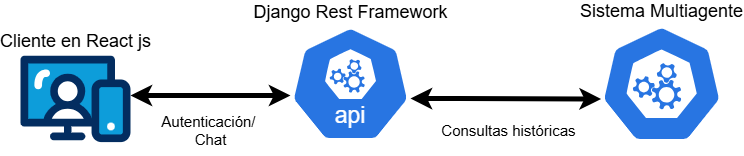
\includegraphics[width=0.9\textwidth]{images/micro.png} 
	\caption{Estructura de la propuesta de solución (Fuente: elaboración propia).}
	\label{fig:arquitectura_web}
\end{figure}

La Figura \ref{fig:arquitectura_web} ilustra la arquitectura general. El flujo de interacción del usuario es el siguiente:

\begin{enumerate}
	\item El usuario interactúa con la interfaz web desarrollada en \textit{React}, donde ingresa sus consultas en lenguaje natural (e.g., “¿Qué barcos llegaron de Europa en enero de 1850?”).
	\item El \textit{frontend} \textit{React} envía la consulta del usuario, típicamente como una petición HTTPS, al \textit{endpoint} correspondiente del \textit{backend} de DRF.
	\item El \textit{backend} de DRF actúa como orquestador principal de la lógica de negocio. Puede gestionar autenticación de usuarios (si aplica), almacenar historial de conversaciones, y, crucialmente, procesa la solicitud entrante. Determina que la consulta requiere procesamiento por IA y la reenvía al microservicio del sistema multiagente a través de una llamada API.
	\item El microservicio del sistema multiagente recibe la consulta y ejecuta su lógica interna basada en agentes para procesar el lenguaje natural, buscar en la base de datos vectorial del \textit{Diario de la Marina}, contextualizar la información y generar la respuesta (texto y/o imágenes).
	\item El microservicio del sistema multiagente devuelve el resultado procesado al \textit{backend} de DRF.
	\item El \textit{backend} de DRF recibe la respuesta del microservicio, la formatea si es necesario (e.g., preparándola para la visualización), y la envía de vuelta al frontend React.
	\item Finalmente, el \textit{frontend React} recibe la respuesta del \textit{backend} de DRF y la presenta al usuario de forma clara y ordenada en la interfaz de chat, mostrando el texto y/o las imágenes generadas.
\end{enumerate}

Dentro del microservicio sistema multiagente opera la lógica conversacional avanzada, cuyo flujo interno se detalla a continuación y se ilustra en la Figura \ref{fig:flujo_mas_interno}. Este microservicio está diseñado específicamente para transformar los datos históricos no estructurados del \textit{Diario de la Marina} en conocimiento estructurado y accesible, superando las limitaciones de herramientas previas mediante la integración de LLMs\footnote{LLM (Large Language Model): Modelo de lenguaje de gran tamaño entrenado con enormes volúmenes de datos textuales, capaz de comprender y generar lenguaje natural con un alto nivel de coherencia, usado en tareas como la traducción automática, el resumen de textos o la generación de respuestas conversacionales.}, RAG\footnote{RAG (Retrieval-Augmented Generation): Técnica que combina modelos generativos con mecanismos de recuperación de información, permitiendo al modelo acceder a fuentes externas relevantes durante la generación de respuestas, mejorando así la precisión y actualidad de los resultados producidos.} y una coordinación eficiente entre agentes especializados.

\begin{figure}[htbp] 
	\centering
	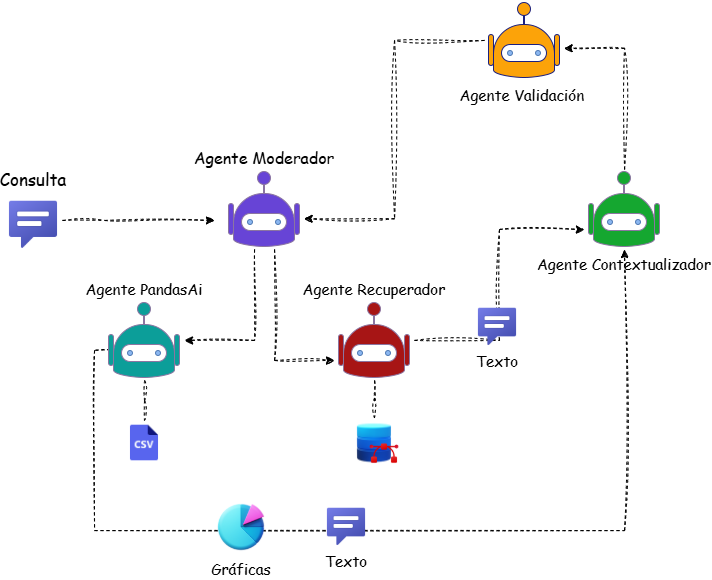
\includegraphics[width=1\textwidth]{images/mas-final.png} 
	\caption{Flujo Interno del Microservicio Multiagente Conversacional (Fuente: elaboración propia).}
	\label{fig:flujo_mas_interno}
\end{figure}

El proceso interno del microservicio (Figura \ref{fig:flujo_mas_interno}) inicia cuando recibe una consulta del \textit{backend} DRF. Esta consulta es manejada por el Agente Moderador, que actúa como coordinador central dentro del microservicio. El Agente Moderador extrae palabras clave (e.g., “barcos”, “Europa”, “enero 1850”) y determina la intención del usuario. En la mayoría de los casos, delega la tarea de búsqueda al Agente PandasAi, que realiza la extracción de datos estructurados (como fechas, nombres de capitanes, puertos) desde el archivo CSV que contiene los datos procesados del \textit{Diario de la Marina}. Solo en casos específicos, cuando la consulta requiere información detallada sobre el contenido de la carga de los barcos, el Agente Moderador coordina con el Agente Recuperador, que convierte las palabras clave en \textit{embeddings} y consulta la base de datos vectorial especializada para recuperar fragmentos relevantes. Los datos recuperados, ya sea por el Agente PandasAi o el Agente Recuperador, se devuelven al Agente Moderador.
Posteriormente, el Agente Moderador envía la información recuperada, junto con la intención del usuario, al Agente Contextualizador. Este agente evalúa si se necesita una respuesta textual, una visualización gráfica (e.g., un gráfico de la frecuencia de llegada de barcos por mes), o ambas. Si se requieren gráficos, el Agente Contextualizador genera instrucciones que se envían al Agente PandasAi. Este agente crea un script Python para generar la visualización, valida su corrección y genera una imagen (e.g., PNG). La imagen resultante se retorna al Agente Contextualizador. Si no se requieren gráficos, el Agente Contextualizador enriquece la información textual. Antes de enviar la respuesta final al \textit{backend} DRF, el Agente Validacion revisa la coherencia y precisión del contenido generado (texto y/o imagen), comparándolo con la consulta original. Finalmente, el Agente Moderador ensambla la respuesta validada y la retorna como salida del microservicio.
Esta arquitectura desacoplada, combinando una interfaz web moderna, un \textit{backend} robusto y un microservicio especializado en IA, no solo facilita la interacción del usuario y la gestión de datos, sino que también optimiza la investigación histórica, contribuye a la preservación del patrimonio documental y permite escalar los componentes de IA de forma independiente.


\section{Análisis de requisitos}

El análisis de requisitos da como resultado la especificación de las características operativas del software. Indica la interfaz de este y otros elementos del sistema, y establece las restricciones que limitan al software \cite{pressman2010practitioner}.Es una fase crucial en el proceso de desarrollo de software. Se trata de una etapa inicial en la cual un analista busca entender las necesidades del cliente y traducirlas en un conjunto de requisitos claros y bien definidos \cite{palli2023analisis}.

\subsection{Técnicas de captura de requisitos}

La definición de los requisitos del sistema se fundamenta en un proceso sistemático de captura, basado en dos técnicas ampliamente reconocidas en ingeniería de software: la entrevista y la observación, aplicadas en el contexto de los ejemplos analizados en el estado del arte (Capítulo 1). Estas técnicas, permitieron identificar las expectativas de los usuarios potenciales y las limitaciones de las soluciones existentes, asegurando que los requisitos reflejen tanto las demandas prácticas como las carencias técnicas observadas~\cite{sommerville2011software}.

\textbf{Entrevista:} Se realizaron entrevistas semiestructuradas con historiadores y académicos especializados en historia del Caribe, quienes serían usuarios finales del sistema. Las preguntas se diseñaron para explorar sus necesidades al interactuar con documentos históricos digitalizados, como el \textit{Diario de la Marina}. Por ejemplo, se les consultó: ``¿Qué tipo de información busca con mayor frecuencia en archivos históricos?'' y ``¿Qué dificultades encuentra al analizar datos marítimos de textos antiguos?''. Las respuestas destacaron la importancia de obtener respuestas contextualizadas (e.g., vinculadas a eventos históricos), la necesidad de visualizaciones gráficas para patrones comerciales y la frustración con errores de transcripción que dificultan el análisis. Estas aportaciones guiaron la definición de requisitos como la corrección de datos y la generación de gráficos.

\textbf{Análisis de Sistema Homólogos:} Mediante el análisis de sistemas existentes es
posible estudiar aplicaciones similares a la que se necesita obtener. Cuando se tiene
la concepción del funcionamiento de un software similar en cuanto a funcionalidades
y características es más sencillo identificar los requisitos del sistema que se necesita
implementar. Durante la investigación se realizó un estudio de aplicaciones similares
a la solución a desarrollar, en las cuales se observaron los diseños de sus interfaces,
las funcionalidades que ofrecen, el grado de dificultad a la hora de interactuar con
la aplicación, entre otros rasgos importantes que contribuyeran a obtener un
producto con la mejor calidad posible~\cite{sommerville2011software}. Como fuente importante
para la obtención de requisitos principales del sistema a desarrollar, se encuentra el
análisis a fondo de los sistemas homólogos estudiados y antes descritos en el
epígrafe 1.7.\\
La combinación de entrevistas y observación permitió comprender las necesidades de los usuarios con las deficiencias técnicas de las soluciones actuales, proporcionando una base sólida para los requisitos funcionales y no funcionales que se detallan a continuación.



\subsection{Requisitos funcionales}

Son declaraciones de los servicios que debe proporcionar el sistema, de la manera en que
éste debe reaccionar a entradas particulares y de cómo se debe comportar en situaciones
particulares. En algunos casos, los requerimientos funcionales de los sistemas también
pueden declarar explícitamente lo que el sistema no debe hacer~\cite{sommerville2011software}.

A continuación, se describen los requisitos funcionales específicos para el sistema multiagente conversacional propuesto:

\begin{longtable}{@{}l >{\raggedright\arraybackslash}p{4.5cm} >{\raggedright\arraybackslash}p{6.5cm} l l@{}} % Ajustados anchos
	\caption{Tabla de Requisitos Funcionales (RF)} \label{tab:requisitos_funcionales_final} \\ 
	\toprule
	\textbf{ID} & \textbf{Nombre} & \textbf{Descripción} & \textbf{Complejidad} & \textbf{Prioridad} \\ 
	\midrule
	\endfirsthead 
	
	\caption[]{Tabla de Requisitos Funcionales (RF) (Continuación)} \\ 
	\toprule
	\textbf{ID} & \textbf{Nombre} & \textbf{Descripción} & \textbf{Complejidad} & \textbf{Prioridad} \\ 
	\midrule
	\endhead 
	
	\bottomrule
	\multicolumn{5}{r@{}}{\textit{Continúa en la siguiente página...}} \\ 
	\endfoot 
	
	\bottomrule
	\endlastfoot 
	
	% --- Gestión de Usuarios y Autenticación ---
	\textbf{RF 1} & Registrar usuario & Permitir a un visitante registrarse proporcionando datos válidos (e.g.,nombre de usuario, email, contraseña), que serán almacenados de forma segura por el \textit{backend}. & Media & Alta \\ 
	\textbf{RF 2} & Autenticar usuario & Permitir a un usuario registrado iniciar sesión proporcionando credenciales válidas, verificadas por el \textit{backend}, generando una sesión activa. & Media & Alta \\ 
	\textbf{RF 3} & Cerrar sesión & Permitir al usuario autenticado finalizar su sesión activa en el sistema. & Baja & Media \\ 
	% --- Gestión de Conversaciones ---
	\textbf{RF 4} & Iniciar conversación & Permitir al usuario autenticado crear una nueva sesión de chat independiente de las anteriores. & Baja & Alta \\ % NUEVO
	\textbf{RF 5} & Listar conversación & Mostrar al usuario autenticado una lista de sus conversaciones previas para poder seleccionarlas y revisarlas. & Media & Media \\ % NUEVO
	\textbf{RF 6} & Visualizar conversación & Permitir al usuario seleccionar una conversación de su historial para visualizarla y continuarla. & Media & Media \\ % NUEVO
	\textbf{RF 7} & Eliminar conversación & Permitir al usuario eliminar permanentemente una conversación específica de su historial. & Media & Baja \\ 
	% --- Interfaz y Flujo del Chat ---
	\textbf{RF 8} & Insertar consulta & Permitir al usuario escribir y enviar una consulta en lenguaje natural dentro de la conversación activa. & Baja & Alta \\ 
	\textbf{RF 9} & Visualizar mensajes & Mostrar de forma clara y ordenada el diálogo (consultas del usuario y respuestas del sistema) dentro de la conversación activa. & Media & Alta \\  
	% --- Procesamiento Interno del Microservicio MAS ---
	\textbf{RF 10} & Recibir consulta & El microservicio MAS debe recibir la consulta para iniciar el flujo de agentes. & Media & Alta \\ 
	\textbf{RF 11} & Analizar consulta & El Agente Moderador debe analizar la consulta para identificar términos clave relevantes. & Alta & Alta \\ 
	\textbf{RF 12} & Determinar acción & El Agente Moderador debe interpretar el propósito principal de la consulta del usuario para determinar la próxima acción del sistema (información, análisis,gráficas estadísticas). & Alta & Alta \\ 
	\textbf{RF 13} & Generar embeddings & El Agente Recuperador debe convertir las palabras clave en representaciones vectoriales (embeddings) adecuadas para la búsqueda semántica. & Alta & Alta \\ 
	\textbf{RF 14} & Consultar base de datos & El Agente Recuperador debe buscar y obtener fragmentos de texto relevantes del \textit{Diario de la Marina} desde la base de datos vectorial, basándose en los embeddings. & Alta & Alta \\
	\textbf{RF 15} & Consultar CSV & El Agente PandasAi debe buscar y obtener fragmentos de texto relevantes del \textit{Diario de la Marina} desde la base de datos en formato csv. & Alta & Alta \\ 
	\textbf{RF 16} & Contextualizar respuesta & El Agente Contextualizador debe generar una respuesta coherente en lenguaje natural, integrando la información recuperada y añadiendo contexto histórico si es pertinente. & Alta & Alta \\ 
	\textbf{RF 17} & Identificar estadísticas & El Agente Contextualizador debe determinar si la consulta o los datos recuperados justifican la creación de una representación gráfica. & Media & Media \\ 
	\textbf{RF 18} & Formular instrucciones para gráfico & Si se requiere un gráfico, el Agente Contextualizador debe generar las especificaciones (tipo de gráfico, datos a usar) para el Agente PandasAi. & Alta & Alta \\ 
	\textbf{RF 19} & Generar script & El Agente PandasAI debe crear un script ejecutable que produzca la visualización solicitada a partir de los datos y especificaciones. & Alta & Alta \\ 
	\textbf{RF 20} & Validar script & El Agente PandasAi debe verificar que el script generado es sintácticamente correcto y no contiene errores obvios antes de ejecutarlo. & Alta & Alta \\ 
	\textbf{RF 21} & Generar imagen & El Agente PandasAi debe ejecutar el script validado para generar la visualización como un archivo de imagen (e.g., PNG, JPG). & Alta & Alta \\ 
	\textbf{RF 22} & Combinar resultados & El Agente Contextualizador (o Moderador) debe combinar la respuesta textual y/o la imagen generada en una estructura de respuesta unificada. & Alta & Alta \\ 
	\textbf{RF 23} & Validar respuesta & El Agente de Validación debe revisar la respuesta preliminar para asegurar su precisión, coherencia con la consulta y ausencia de información errónea. & Alta & Alta \\  
	\textbf{RF 24} & Enviar respuesta & El microservicio MAS debe enviar la respuesta final ensamblada al \textit{backend} a través de su API. & Media & Alta \\ 
	% --- Flujo de Respuesta Backend y Frontend ---
	\textbf{RF 25} & Visualizar respuesta & El \textit{backend} debe enviar la respuesta (texto y/o referencia a la imagen) al \textit{frontend} para su visualización. & Media & Alta \\ 
	
\end{longtable}

\subsection{Requisitos no funcionales}

Los requisitos no funcionales son aquellos que no se refieren directamente a las funciones
específicas que proporciona el sistema, sino a las propiedades de este como fiabilidad,
tiempo de respuesta y la capacidad de almacenamiento. Incluyen además restricciones de
tiempo, sobre el proceso de desarrollo y estándares~\cite{sommerville2011software}.
A continuación, se definen los requisitos no funcionales que debe cumplir la aplicación
basándose en los establecido por las normas ISO 25000 Calidad del Producto de Software,
específicamente la ISO/IEC 25010 que define las características de calidad que se tienen
en cuenta al evaluar las propiedades de un producto de software~\cite{ISO25010-2023}.
A continuación, se listan los requisitos no funcionales identificados:

\begin{longtable}{@{}p{2cm}p{12cm}@{}}
	\caption{Requisitos No Funcionales (RNF)} \label{tab:rnf_iso25010} \\
	\toprule
	\textbf{ID} & \textbf{Descripción} \\
	\midrule
	\endfirsthead
	
	\caption[]{Requisitos No Funcionales (RNF) (continuación)} \\
	\toprule
	\textbf{ID} & \textbf{Descripción} \\
	\midrule
	\endhead
	
	\bottomrule
	\endfoot
	
	% --- RENDIMIENTO ---
	\multicolumn{2}{@{}l}{\textbf{RNF 1: Rendimiento}} \\[0.5ex]
	RNF 1.1 & Tiempo de respuesta para consultas simples (búsqueda de barcos por nombre o fecha) no superior a los 30 segundos para 20 usuarios concurrentes. \\
	RNF 1.2 & Tiempo de respuesta para consultas complejas con generación de gráficos no superior a un minuto para 20 usuarios concurrentes. \\
	\addlinespace
	
	% --- SEGURIDAD ---
	\multicolumn{2}{@{}l}{\textbf{RNF 2: Seguridad}} \\[0.5ex]
	RNF 2.1 & Almacenamiento seguro de contraseñas de usuarios \\
	RNF 2.2 & Rastreabilidad de decisiones tomadas por los agentes IA \\
	RNF 2.3 & El acceso a la información debe estar restringido por usuario, contraseña.\\
	\addlinespace
	
	% --- USABILIDAD ---
	\multicolumn{2}{@{}l}{\textbf{RNF 3: Usabilidad}} \\[0.5ex]
	RNF 3.1 & Retroalimentación visual durante el procesamiento de consultas \\
	RNF 3.2 & Mensajes de error claros y comprensibles para usuarios \\
	\addlinespace
	
	% --- FIABILIDAD ---
	\multicolumn{2}{@{}l}{\textbf{RNF 4: Fiabilidad}} \\[0.5ex]
	RNF 4.1 & Alta disponibilidad del sistema completo \\
	RNF 4.2 & El sistema debe ser tolerante a fallos, y mostrar solo la información necesaria para orientar al usuario\\
	\addlinespace
		
	% --- MANTENIBILIDAD ---
	\multicolumn{2}{@{}l}{\textbf{RNF 5: Mantenibilidad}} \\[0.5ex]
	RNF 5.1 & El software estará bien documentado de forma tal que el tiempo de mantenimiento
	sea mínimo en caso de necesitarse. \\
	RNF 5.2 & Se debe hacer uso de los estándares de codificación definidos para el sistema multiagente \\
	RNF 5.3 & Gestión controlada de dependencias \\
	\addlinespace
	
\end{longtable}


\subsection{Historias de usuarios}

Las historias de usuario (HU) son descripciones breves y simples de los requerimientos de un cliente o usuario, que facilitan la comunicación con los desarrolladores del proyecto. Estas historias permiten expresar las expectativas y necesidades de los usuarios de una manera clara y comprensible, evitando ambigüedades y malentendidos que podrían llevar a pérdidas de tiempo y recursos \cite{menzinsky2018historias}.

Se realiza una HU por cada requisito funcional, a continuación, se mostrarán las HU más relevantes. Para consultar el resto de las historias de usuario, se remite al \textbf{Anexo A}, donde se presentan de forma completa y organizada. Estas historias complementan la visión general del sistema y permiten una comprensión más exhaustiva de los requerimientos funcionales detallados.

% ==========================================
% Funcionalidad Principal del Chat y MAS
% ==========================================

\begin{userstory}[hu:08]
	\storyname{Interactuar con el chat activo (Enviar Consulta y Ver Respuesta)}
	\storyuser{Usuario autenticado}
	\storyiter{1} % Iteración ajustada
	\storypriority{Alta} % Basado en RF9 (Input), RF10, RF26, RF27, RF28
	\storyrisk{Medio} % Riesgo en la comunicación FE-BE-MAS
	\storypoints{2 semanas} % Estimación ajustada (cubre FE y BE básico)
	\storyprogrammer{Daniel Rojas Grass}
	\storydescription{
		Como usuario autenticado, puede escribir una consulta en lenguaje natural en la interfaz de chat, enviarla al sistema, y ver tanto su consulta como la respuesta del sistema (texto y/o imagen) mostradas de forma clara y ordenada en el área de diálogo de la conversación activa. (Corresponde principalmente a RF9-Input, RF10, RF26, RF27, RF28)
		
		\textbf{Precondiciones:}
		\begin{itemize}
			\item El usuario tiene una sesión activa.
			\item El usuario tiene una conversación activa (nueva HU:04 o cargada HU:06).
			\item El \textit{frontend}, el \textit{backend} y el microservicio MAS están operativos y pueden comunicarse entre sí.
		\end{itemize}
		
		\textbf{Flujo de acción:}
		\begin{enumerate}
			\item Usuario escribe una consulta en el campo de texto del chat.
			\item Usuario envía la consulta (click en botón 'Enviar' o presiona 'Enter').
			\item El \textit{frontend} muestra inmediatamente la consulta del usuario en el área de diálogo (marcada como del usuario).
			\item El \textit{frontend} envía la consulta y el ID de la conversación activa (si existe) al \textit{backend}.
			\item (Flujo cubierto en HU:09 y HU:10) El \textit{backend} recibe la consulta, la envía al microservicio MAS para procesamiento, recibe la respuesta del MAS (texto y/o referencia a imagen) y la almacena en la BD asociada a la conversación (RF9-Persistencia).
			\item El \textit{backend} envía la respuesta procesada (texto y/o URL/datos de imagen) al frontend.
			\item El \textit{frontend} recibe la respuesta del \textit{backend}.
			\item El \textit{frontend} muestra la respuesta del sistema (texto y/o imagen) en el área de diálogo (marcada como del sistema).
		\end{enumerate}
	}
	\storyobservation{
		La interfaz debe indicar visualmente cuándo el sistema está procesando la respuesta. El manejo de errores (fallos de red, errores del MAS) debe ser robusto, mostrando mensajes apropiados al usuario. La visualización del chat debe permitir navegar para ver mensajes antiguos.
	}
	\storyinterface{Interfaz principal del Chat en el sitio web mostrando diálogo:
		\par\medskip % Añade un pequeño espacio vertical
		\begin{center} % Para centrar la imagen
			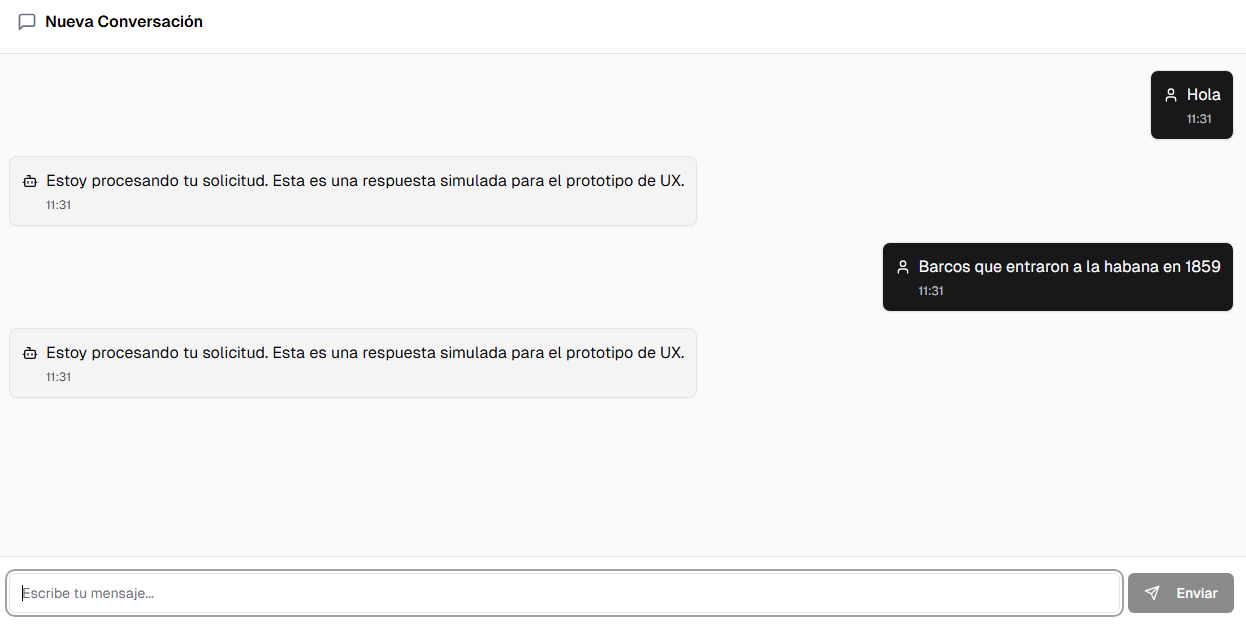
\includegraphics[width=0.6\textwidth]{images/chat.PNG} % Imagen del ejemplo
		\end{center}
		\medskip
	}
	
\end{userstory}

\begin{userstory}[hu:09]
	\storyname{Obtener respuesta textual relevante del MAS}
	\storyuser{Usuario autenticado (indirectamente, a través del sistema)}
	\storyiter{2} % Iteración estimada
	\storypriority{Alta} % Basado en RF11-16, RF22-25
	\storyrisk{Alto} % Riesgo asociado a la calidad/precisión de la IA
	\storypoints{4 semanas} % Estimación basada en ejemplo (complejidad alta)
	\storyprogrammer{Daniel Rojas Grass}
	\storydescription{
		Como sistema, consulta el microservicio MAS para que procese la consulta recibida del \textit{backend}, la analice (palabras clave, intención), recupere información relevante del \textit{Diario de la Marina} desde la BD vectorial, sintetice una respuesta textual coherente y contextualizada, la valide y la devuelva al \textit{backend}, para que el usuario final reciba información precisa. (Corresponde al flujo interno del MAS: RF11, RF12, RF13, RF14, RF15, RF16, RF22, RF23, RF24, RF25)
		
		\textbf{Precondiciones:}
		\begin{itemize}
			\item El microservicio MAS (\textit{FastApi}) está operativo.
			\item Todos los agentes internos (Moderador, Pandasai, Contextualizador, Validación) están implementados y disponibles.
			\item La base de datos vectorial (Faiss) está cargada con los datos del *Diario de la Marina* y es accesible.
			\item El csv con los datos del \textit{Diario de la Marina} esta cargado y es accesible.
			\item El LLM subyacente está configurado y accesible.
			\item El MAS recibe una solicitud válida del \textit{backend} a través de su API.
		\end{itemize}
		
		\textbf{Flujo de acción (interno del MAS):}
		\begin{enumerate}
			\item MAS recibe la consulta vía \textit{API REST} (RF11).
			\item Agente Moderador extrae palabras clave y determina intención (RF12, RF13).
			\item Agente Recuperador genera \textit{embeddings} y busca en BD vectorial (RF14, RF15).
			\item Agente PandasAi genera tanto gráficas como búsquedas de análisis en el csv.
			\item Agente Contextualizador recibe fragmentos relevantes y genera respuesta textual inicial, añadiendo contexto (RF16).
			\item (Si no se requiere gráfico) Agente Contextualizador (o Moderador) prepara la respuesta textual preliminar (RF22).
			\item Agente Validación revisa coherencia, relevancia y posible toxicidad/error (RF23).
			\item Agente Moderador ensambla la respuesta textual validada en formato JSON (RF24).
			\item MAS retorna la respuesta JSON al \textit{backend DRF} (RF25).
		\end{enumerate}
	}
	\storyobservation{
		La calidad de los embeddings y la estrategia de recuperación son críticas (RF14, RF15). La capacidad del LLM para sintetizar y contextualizar es fundamental (RF16). El agente de validación es clave para la fiabilidad (RF23). La latencia del proceso completo debe ser aceptable (considerar RNF).
	}
	\storyinterface{[N/A - Proceso interno del Microservicio MAS]}
	
\end{userstory}

\begin{userstory}[hu:10]
	\storyname{Recibir visualización gráfica cuando sea pertinente}
	\storyuser{Usuario autenticado}
	\storyiter{3} % Iteración estimada
	\storypriority{Media} % Basado en RF17-21
	\storyrisk{Moderado} % Riesgo en la generación y validación del script/gráfico
	\storypoints{2 semanas} % Estimación basada en ejemplo (complejidad alta)
	\storyprogrammer{Daniel Rojas Grass}
	\storydescription{
		Como usuario autenticado, cuando la consulta o la información recuperada sugieran la necesidad de una visualización (e.g., análisis de tendencias, comparación de datos), el sistema (específicamente el MAS) genera un gráfico apropiado (e.g., barras, líneas) se debe presentar como una imagen dentro de la respuesta del chat, junto con el texto explicativo, para facilitar la comprensión del usuario. (Corresponde principalmente a RF17, RF18, RF19, RF20, RF21, RF22-integración, RF28-visualización)
		
		\textbf{Precondiciones:}
		\begin{itemize}
			\item El flujo de HU:09 está en progreso.
			\item El Agente Contextualizador identifica que la consulta/datos justifican un gráfico (RF17).
			\item Los datos necesarios para el gráfico están disponibles y estructurados.
			\item El Agente PandasAi listo para la generación de gráficas.
		\end{itemize}
		
		\textbf{Flujo de acción (continuación de HU:09):}
		\begin{enumerate}
			\item Agente Contextualizador determina necesidad de gráfico y formula instrucciones (tipo, datos) (RF17, RF18).
			\item Agente Contextualizador invoca al Agente PandasAi con las instrucciones.
			\item Agente PandasAi genera el script de Pandas para crear el gráfico (RF19).
			\item Agente PandasAi valida la sintaxis y lógica básica del script (RF20).
			\item Agente PandasAi ejecuta el script validado para generar la imagen del gráfico (e.g., PNG) (RF21).
			\item Agente PandasAi devuelve la imagen (o una referencia a ella) al Agente Contextualizador/Moderador.
			\item Agente Contextualizador/Moderador integra la imagen junto con la respuesta textual en la estructura preliminar (RF22).
			\item (Continúa flujo de HU:09) Validación (RF23), Ensamblaje (RF24), Retorno al \textit{backend} (RF25).
			\item (Flujo de HU:08) \textit{Backend} envía URL/datos de imagen al \textit{frontend}.
			\item \textit{Frontend} muestra la imagen recibida dentro del chat (RF28).
		\end{enumerate}
	}
	\storyobservation{
		La detección de la necesidad de un gráfico debe ser fiable (RF17). La generación del script debe ser segura (evitar ejecución de código arbitrario). La validación del script (RF20) es importante para evitar errores en tiempo de ejecución. Los gráficos deben ser claros y legibles. Considerar formatos de imagen web-friendly (PNG, JPG, SVG).
	}
	\storyinterface{Visualización de imagen (gráfico) dentro del Chat en el sitio web, junto al texto explicativo.}
	
\end{userstory}

Las historias de usuario presentadas detallan los requerimientos funcionales del sistema desde la perspectiva del usuario, abarcando desde la gestión de usuarios y autenticación hasta la interacción con el chat y la generación de respuestas textuales y gráficas por parte del microservicio MAS. Estas historias no solo especifican el comportamiento esperado del sistema, sino que también establecen una base clara para el diseño y desarrollo del software, asegurando que las necesidades del usuario se traduzcan en funcionalidades concretas.



\subsection{Tarjetas CRC}

Las tarjetas CRC (Clase-Responsabilidad-Colaboración) son una herramienta de diseño de software orientado a objetos, creada por Kent Beck y Ward Cunningham. Estas tarjetas se utilizan para identificar las clases, sus responsabilidades y cómo colaboran con otras clases para cumplir tareas específicas en un sistema \cite{BeckCunningham}. La representación del sistema multiagente y su interfaz gráfica mediante tarjetas CRC permite estructurar de forma clara y concisa las clases que lo componen, sus responsabilidades específicas y las colaboraciones necesarias para cumplir sus objetivos. Esta técnica facilita la comprensión del comportamiento de cada agente dentro del sistema —como el coordinador, el buscador de información o el generador de respuestas—, promoviendo un diseño orientado a objetos coherente, reutilizable y fácil de mantener. Además, al emplearse en etapas tempranas del desarrollo, las tarjetas CRC fortalecen la comunicación entre desarrolladores y respaldan la validación del modelo antes de su implementación definitiva.

\begin{longtable}{|l|l|}
	\caption{Tarjeta CRC: Agente Moderador} \label{tablacrc1} \\
	
	\hline
	\multicolumn{2}{|c|}{\textbf{Tarjeta CRC}} \\
	\hline
	\textbf{Clase} & \textbf{Agente Moderador} \\
	\hline
	\endfirsthead
	
	\hline
	\textbf{Responsabilidad} & \textbf{Colaboración} \\
	\hline
	\endhead
	
	\hline
	\multicolumn{2}{|r|}{Continúa en la próxima página} \\
	\hline
	\endfoot
	
	\hline
	\endlastfoot
	
	\parbox[t]{0.45\linewidth}{\textbf{Responsabilidades:} \\ 
		Recibir la consulta del usuario \\ 
		Extraer palabras clave e identificar la intención \\ 
		Coordinar el flujo de información entre agentes \\ 
		Ensamblar y entregar la respuesta final al usuario} 
	& 
	\parbox[t]{0.45\linewidth}{\textbf{Colaboración:} \\
		Agente PandasAi \\ 
		Agente recuperador de información (FAISS)\\
		Agente Contextualizador \\ 
		Agente de Validación}
\end{longtable}


\begin{longtable}{|l|l|}
	\caption{Tarjeta CRC: Agente recuperador de información (FAISS) } \label{tablacrc2} \\
	
	\hline
	\multicolumn{2}{|c|}{\textbf{Tarjeta CRC}} \\
	\hline
	\textbf{Clase} & \textbf{Agente recuperador de información (FAISS)} \\
	\hline
	\endfirsthead
	
	\hline
	\textbf{Responsabilidad} & \textbf{Colaboración} \\
	\hline
	\endhead
	
	\hline
	\multicolumn{2}{|r|}{Continúa en la próxima página} \\
	\hline
	\endfoot
	
	\hline
	\endlastfoot
	
	\parbox[t]{0.45\linewidth}{\textbf{Responsabilidades:} \\ 
		Convertir las palabras clave en \textit{embeddings} \\ 
		Consultar la base de datos vectorial para recuperar la información relevante \\ 
		Devolver los resultados al Agente Moderador} 
	& 
	\parbox[t]{0.45\linewidth}{\textbf{Colaboración:} \\
		Agente Moderador \\ 
		Base de datos vectorial}
\end{longtable}

\begin{longtable}{|l|l|}
	\caption{Tarjeta CRC: Agente Contextualizador} \label{tablacrc3} \\
	
	\hline
	\multicolumn{2}{|c|}{\textbf{Tarjeta CRC}} \\
	\hline
	\textbf{Clase} & \textbf{Agente Contextualizador} \\
	\hline
	\endfirsthead
	
	\hline
	\textbf{Responsabilidad} & \textbf{Colaboración} \\
	\hline
	\endhead
	
	\hline
	\multicolumn{2}{|r|}{Continúa en la próxima página} \\
	\hline
	\endfoot
	
	\hline
	\endlastfoot
	
	\parbox[t]{0.45\linewidth}{\textbf{Responsabilidades:} \\ 
		Recibir la información relevante y la intención del usuario \\ 
		Generar indicaciones de estadísticas o contextualizar la información según la petición del usuario \\ 
		Enviar la información procesada al Agente Moderador} 
	& 
	\parbox[t]{0.45\linewidth}{\textbf{Colaboración:} \\
		Agente Moderador \\ 
		Agente PandasAi}
\end{longtable}


\begin{longtable}{|l|l|}
	\caption{Tarjeta CRC: Agente de Validación} \label{tablacrc4} \\
	
	\hline
	\multicolumn{2}{|c|}{\textbf{Tarjeta CRC}} \\
	\hline
	\textbf{Clase} & \textbf{Agente de Validación} \\
	\hline
	\endfirsthead
	
	\hline
	\textbf{Responsabilidad} & \textbf{Colaboración} \\
	\hline
	\endhead
	
	\hline
	\multicolumn{2}{|r|}{Continúa en la próxima página} \\
	\hline
	\endfoot
	
	\hline
	\endlastfoot
	
	\parbox[t]{0.45\linewidth}{\textbf{Responsabilidades:} \\ 
		Revisar la coherencia de la respuesta generada por el sistema \\ 
		Comparar la respuesta con la entrada original \\ 
		Validar o rechazar la respuesta antes de enviarla al usuario} 
	& 
	\parbox[t]{0.45\linewidth}{\textbf{Colaboración:} \\
		Agente Moderador \\ 
		Agente Contextualizador}
\end{longtable}

\begin{longtable}{|l|l|}
	\caption{Tarjeta CRC: Agente PandasAi} \label{tablacrc5} \\
	
	\hline
	\multicolumn{2}{|c|}{\textbf{Tarjeta CRC}} \\
	\hline
	\textbf{Clase} & \textbf{Agente PandasAi} \\
	\hline
	\endfirsthead
	
	\hline
	\textbf{Responsabilidad} & \textbf{Colaboración} \\
	\hline
	\endhead
	
	\hline
	\multicolumn{2}{|r|}{Continúa en la próxima página} \\
	\hline
	\endfoot
	
	\hline
	\endlastfoot
	
	\parbox[t]{0.45\linewidth}{\textbf{Responsabilidades:} \\ 
		Generar un \textit{script} de Pandas para representar estadísticas gráficas cuando sea necesario \\ 
		Validar el \textit{script} y asegurarse de que sea correcto \\ 
		Convertir el gráfico generado en una imagen que pueda ser integrada en la respuesta final\\
		Hacer consultas al CSV cargado para hacer análisis profundos de datos.} 
	& 
	\parbox[t]{0.45\linewidth}{\textbf{Colaboración:} \\
		Agente Contextualizador \\ 
		}
\end{longtable}

En este documento se incluyen ejemplos representativos de algunas de las tarjetas CRC más relevantes para el desarrollo de la solución propuesta. Sin embargo, debido a su extensión, se remite al \textit{Anexo B} para consultar el conjunto completo de las tarjetas CRC, donde se detallan todas las clases identificadas, sus responsabilidades y los colaboradores correspondientes.

\section{Diseño de la propuesta de solución}

\subsection{Diseño de la arquitectura}

La arquitectura propuesta adopta el estilo de microservicios, en el cual la aplicación se descompone en un conjunto de servicios independientes, cada uno ejecutándose en su propio proceso y comunicándose mediante protocolos API REST~\cite{turn0search0}. Cada microservicio se orienta a una capacidad de negocio específica, lo que facilita la comprensión y el mantenimiento aislado de los componentes~\cite{turn0search6,turn0search0}. La modularidad inherente a este enfoque permite el despliegue automatizado e independiente de cada servicio, mejorando la agilidad operativa y reduciendo el tiempo de inactividad asociado a las actualizaciones \cite{turn0search8,turn0search3}. La escalabilidad horizontal se ve potenciada, dado que cada servicio puede replicarse de forma autónoma según la demanda, optimizando el uso de recursos y posibilitando un dimensionamiento granular \cite{turn0search3,turn1search0}. El desacoplamiento entre servicios incrementa la tolerancia a fallos, ya que la interrupción de un componente no compromete la disponibilidad del sistema global \cite{turn0search2,turn0search6}. La heterogeneidad tecnológica está plenamente soportada, puesto que cada microservicio puede implementarse con los lenguajes y \textit{frameworks} más adecuados para su responsabilidad particular \cite{turn0search6,turn1search8}.

\begin{figure}[htbp] 
	\centering
	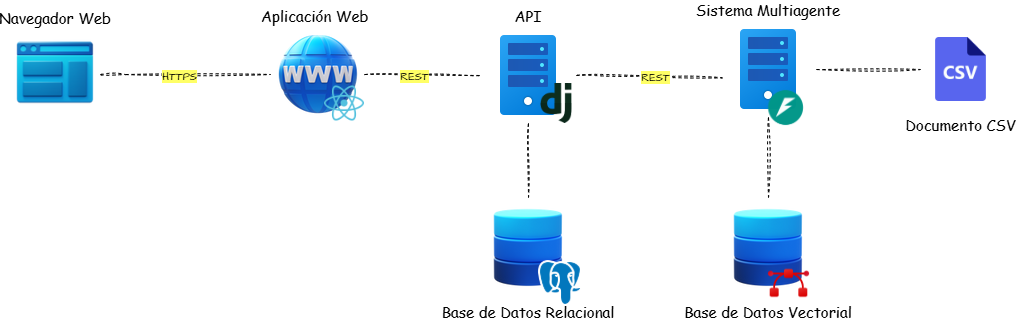
\includegraphics[width=1\textwidth]{images/Arquitectura.png} 
	\caption{Arquitectura de microservicios del sistema multiagente (Fuente: elaboración propia).}
	\label{fig:erquitectura_MAS}
\end{figure}

La presente configuración arquitectónica se materializa en tres componentes principales como se puede visualizar en la Figura \ref{fig:erquitectura_MAS}:
  
\begin{enumerate}
	\item Un \textit{frontend} desarrollado con \textit{React}, encargado de la interacción con el usuario.  
	\item Un \textit{backend} construido con \textit{Django REST Framework}, que actúa como orquestador de la lógica de negocio y gestor de peticiones.  
	\item Un microservicio especializado en procesamiento de lenguaje natural, implementado con \textit{FastApi}, que alberga el sistema multiagente conversacional.  
\end{enumerate}

Esta elección garantiza la independencia en el ciclo de vida de cada servicio, promoviendo la mantenibilidad y facilitando la incorporación de nuevas tecnologías o la sustitución de componentes sin afectar al sistema global \cite{turn0search1,turn1search4}.

\subsubsection{Arquitectura RAG}

Complementando la arquitectura general de microservicios, el Microservicio Multiagente Conversacional implementa internamente un flujo de trabajo basado en la Arquitectura de Generación Aumentada por Recuperación (RAG)\footnote{Un sistema RAG (\textit{Retrieval Augmented Generation}, o Generación Aumentada por Recuperación) es una arquitectura de inteligencia artificial que combina modelos de lenguaje avanzados (LLM) con mecanismos de recuperación de información en tiempo real. Su objetivo es mejorar la precisión, relevancia y actualidad de las respuestas generadas por la IA, permitiéndole acceder a bases de datos o documentos externos que contienen información más reciente o específica que la que fue utilizada durante el entrenamiento del modelo.}~\cite{lewis2020retrievalaugmented}. Esta aproximación es fundamental para que el sistema pueda interactuar de manera precisa y contextualizada con los datos específicos del \textit{Diario de la Marina}.

El proceso RAG dentro del microservicio entra en acción cuando  la consulta requiere información detallada del contenido textual del periódico, entonces el Agente Recuperador utiliza un modelo de embeddings para convertir la consulta del usuario en una representación vectorial, realiza una búsqueda de similitud en la base de datos vectorial (FAISS), que contiene los embeddings de los fragmentos de texto del \textit{Diario de la Marina} donde recupera los fragmentos de texto más relevantes semánticamente para la consulta y los envía al siguiente agente en la cadena de procesamiento como se observa en la Figura \ref{fig:rag}.

\begin{figure}[htbp] 
	\centering
	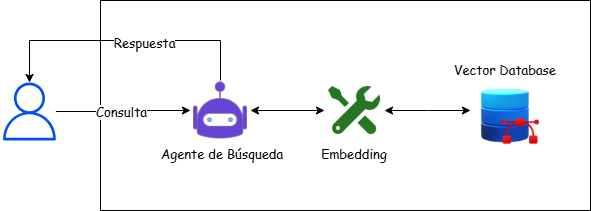
\includegraphics[width=0.5\textwidth]{images/RAGArchitect.png} 
	\caption{Arquitectura RAG (Fuente: elaboración propia).}
	\label{fig:rag}
\end{figure}

\subsection{Diseño del modelo de datos}

\begin{figure}[htbp] 
	\centering
	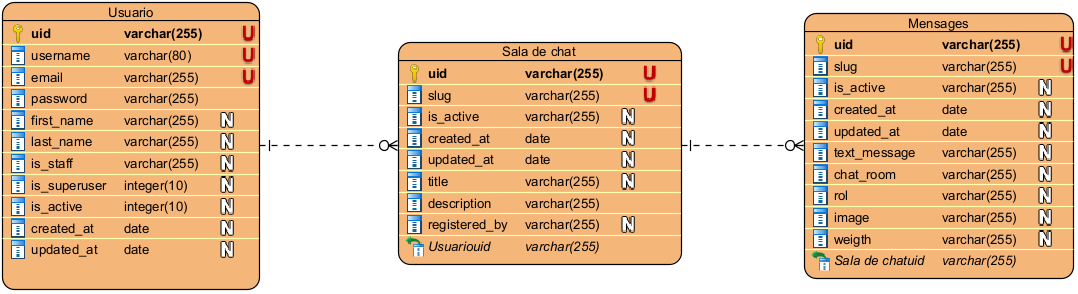
\includegraphics[width=1\textwidth]{images/modelo.png} 
	\caption{Diseño del modelo de datos (Fuente: elaboración propia).}
	\label{fig:modelo_de_datos}
\end{figure}


El modelo de datos propuesto en la Figura \ref{fig:modelo_de_datos} articula de manera coherente la estructura relacional necesaria para soportar un sistema de chat en tiempo real~\cite{Codd1970}. Se fundamenta en los principios del modelo relacional que establecen las bases para el almacenamiento y la recuperación eficiente de datos, garantizando la unicidad de las tuplas y la ausencia de redundancia innecesaria~\cite{Silberschatz2019}.\\
La definición de la entidad \textbf{Usuario} contempla un identificador único uid, atributos de autenticación y perfil, así como indicadores de estado y marcas temporales de creación y modificación, satisfaciendo los requerimientos de integridad y auditoría en el dominio de usuario~\cite{ElmasriNavathe2010}. La elección de tipos de datos \textit{VARCHAR} para los campos característicos responde a la flexibilidad necesaria para posibles extensiones en los identificadores y datos personales~\cite{Date2003}.\\
La entidad \textbf{Sala de chat} permite agrupar conversaciones de manera lógica y filtrable~\cite{ConnollyBegg2014}. Al establecer una relación de uno a muchos con la entidad Usuario a través de la clave foránea \textit{registered\_by}, se refuerza la trazabilidad de la creación y administración de espacios de comunicación~\cite{Harrington2015}.\\
La entidad \textbf{Mensajes} está diseñada para almacenar cada mensaje asociado a una sala de chat, con su propio identificador, estado de actividad, contenido textual, atributos de rol y metadatos adicionales que facilitan la moderación y la representación multimodal~\cite{Silberschatz2019}. La implementación de la clave foránea \textit{chat\_room} garantiza la integridad referencial, evitando mensajes huérfanos y asegurando la coherencia de las interacciones~\cite{IBMReferential}.\\
El diseño enfatiza la normalización hasta la tercera forma normal, minimizando anomalías de actualización y duplicación de datos~\cite{Silberschatz2019}. Asimismo, la adopción de métodos ágiles para el modelado de datos respalda iteraciones rápidas y adaptativas durante el ciclo de vida del desarrollo~\cite{Ambler2003}. La adherencia al estándar SQL definido en ISO/IEC 9075 certifica la interoperabilidad en entornos heterogéneos de bases de datos~\cite{ISO9075}.Finalmente, la consideración de criterios de escalabilidad y rendimiento se inspira en lecciones históricas sobre arquitecturas de sistemas de datos~\cite{Stonebraker2005}.


\section{Implementación}

\subsection{Estándares de codificación en Python y JavaScript}

Los estándares de codificación son esenciales para garantizar la mantenibilidad, colaboración y calidad del software~\cite{van2001pep}. En este epígrafe se analiza comparativamente las convenciones principales para Python y JavaScript, destacando sus similitudes y diferencias fundamentales.

\subsubsection{Estándares para Python}

\begin{enumerate}
	\item \textbf{Convenciones de Estilo}: Python cuenta con una guía oficial de estilo denominada PEP 8, que establece directrices precisas para la escritura de código. La indentación de 4 espacios (prohibiendo el uso de tabuladores) y el límite de 79 caracteres por línea son dos de sus reglas más características. El espaciado alrededor de operadores y la organización de \textit{imports} en tres grupos (bibliotecas estándar, terceros y locales) promueven la consistencia visual. La nomenclatura sigue patrones específicos: \texttt{snake\_case} para funciones y variables, \textit{PascalCase} para clases, y \textit{MAYÚSCULAS} para constantes\cite{van2001pep}. La documentación mediante \textit{docstrings} (siguiendo PEP 257~\cite{PEP257}) facilita la generación automática de documentación técnica.
	\item \textbf{Herramientas y Prácticas}: El ecosistema \textit{Python} ofrece herramientas como \textit{flake8} para verificación de estilo y \textit{black} para formateo automático. El uso de \textit{type hints} (desde \textit{Python 3.5}) mejora la seguridad de tipos en proyectos complejos. El manejo de excepciones debe ser explícito, evitando cláusulas \textit{except} genéricas que puedan ocultar errores.
\end{enumerate}

\subsubsection{Estándares para JavaScript}

\begin{enumerate}
	\item \textbf{Guías de Referencia}: JavaScript carece de un estándar oficial único, pero guías como el \textit{Airbnb JavaScript Style Guide}~\cite{AirbnbJS} y \textit{Google JavaScript Style Guide}~\cite{GoogleJS} se han consolidado como referencias. Estas enfatizan el uso de ES6+, con preferencia por \textit{const/let} sobre \textit{var}, y \textit{arrow functions} para \textit{callbacks}.\\
	La convención de nombres utiliza \textit{camelCase} para variables/funciones y \textit{PascalCase} para clases. Los literales de plantilla (\textit{template strings}) son preferidos sobre concatenación manual, y el punto y coma sigue siendo opcional pero debe usarse consistentemente.
	\item \textbf{Ecosistema Moderno}: Herramientas como \textit{ESLint} (configurable con reglas específicas) y \textit{Prettier} automatizan la aplicación de estándares. El sistema de módulos ES6 (\textit{import/export}) ha reemplazado ampliamente a \textit{require} en proyectos nuevos. Para proyectos complejos, TypeScript ofrece tipado estático, reduciendo errores en tiempo de ejecución~\cite{TypeScript}.
\end{enumerate}

Ambos lenguajes comparten principios fundamentales: modularización del código, documentación clara, y uso de linters. Python muestra mayor uniformidad gracias a PEP 8, mientras JavaScript permite más flexibilidad mediante guías configurables. En rendimiento, JavaScript prioriza la compatibilidad con navegadores, mientras Python enfatiza la legibilidad como principio filosófico~\cite{PEP20}. La adopción de estándares debe adaptarse al contexto del proyecto y equipo, utilizando herramientas automatizadas para garantizar cumplimiento. Tanto Python como JavaScript han desarrollado ecosistemas maduros que, cuando se usan consistentemente, elevan sustancialmente la calidad del código.

\subsection{Patrones de diseño}
\label{sec:patrones_diseno}

Los patrones de diseño de software representan soluciones probadas y estandarizadas para problemas recurrentes en el desarrollo, encapsulando mejores prácticas y promoviendo la creación de software modular, legible, flexible y robusto \cite{gavilanez2022analisis}. En el desarrollo de esta aplicación web y su microservicio asociado, se han aplicado conscientemente varios patrones para abordar los desafíos inherentes a su arquitectura distribuida y su flujo de trabajo basado en IA. A continuación, se analizan los patrones de diseño a implementar en el sistema multiagente conversacional y en el \textit{backend} (desarrollado con \textit{Django REST Framework}), destacando su relevancia y su impacto en el procesamiento de datos históricos del \textit{Diario de la Marina}.

\textbf{Patrón Singleton} se utiliza para gestionar recursos críticos compartidos en el sistema multiagente, asegurando que componentes como la base de datos históricos, el índice FAISS para la base de datos vectorial, y los agentes tengan una única instancia en toda la aplicación. Este patrón es fundamental para optimizar el uso de recursos, ya que evita la creación redundante de instancias pesadas, lo que podría impactar negativamente el rendimiento del sistema, especialmente al procesar grandes volúmenes de datos históricos del \textit{Diario de la Marina}. La Figura \ref{fig:codigo_singleton} muestra un extracto de este código, evidenciando la implementación del patrón.\\
La importancia del patrón \textit{Singleton} radica en su capacidad para centralizar el acceso a recursos compartidos, reduciendo la sobrecarga computacional y asegurando consistencia en los datos procesados. Esto es particularmente relevante en un sistema multiagente, donde múltiples agentes (como \texttt{AgenteRecuperador} y \texttt{AgentePandasAi}) necesitan acceder a las mismas estructuras de datos para generar respuestas textuales o gráficas.

\begin{figure}[htbp]
	\centering
	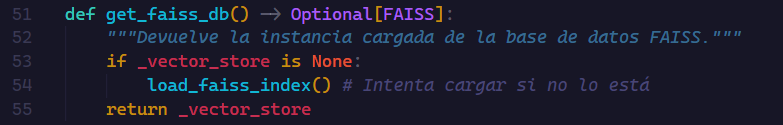
\includegraphics[width=0.8\textwidth]{images/singleton.PNG}
	\caption{Extracto de código que implementa el patrón (Fuente: elaboración propia). \textit{Singleton}.}
	\label{fig:codigo_singleton}
\end{figure}

\textbf{Patrón Cadena de responsabilidad} permite que el sistema multiagente implemente un flujo de trabajo estructurado, que orqueste la ejecución de agentes a través de un grafo de estados. Este patrón permite que cada agente (como el moderador, el contextualizador, el ejecutor PandasAI, y el validador) procese y modifique un estado compartido, pasando el control al siguiente agente en la cadena. Esta estructura es esencial para manejar consultas complejas que requieren el procesamiento conjunto de datos estructurados (del archivo CSV) y no estructurados (de la base vectorial), como se describe en la Figura \ref{fig:codigo_workflow}.\\ 
La relevancia de este patrón radica en su capacidad para modularizar el flujo de procesamiento, permitiendo que cada agente se especialice en una tarea específica. Esto no solo facilita el mantenimiento y la extensibilidad del sistema, sino que también asegura que las consultas se procesen de manera eficiente, cumpliendo con los requisitos funcionales relacionados con la generación de respuestas.

\begin{figure}[htbp]
	\centering
	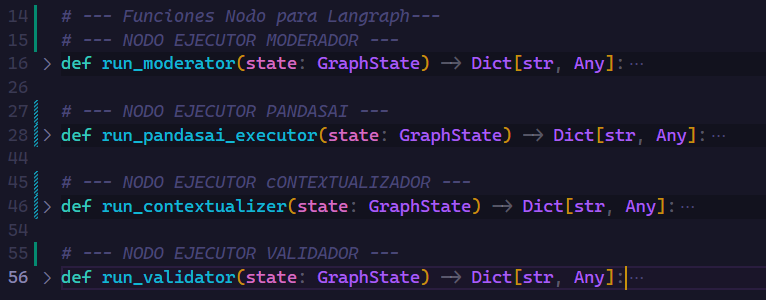
\includegraphics[width=0.8\textwidth]{images/cadena.PNG}
	\caption{Extracto de código que implementa el patrón \textit{Cadena de responsabilidad} (Fuente: elaboración propia).}
	\label{fig:codigo_workflow}
\end{figure}

\textbf{Patrón Plantilla Abstracta} permite estandarizar comportamientos comunes en modelos, serializadores y paginaciones. Este patrón permite definir una estructura general que puede ser heredada y personalizada por clases específicas, promoviendo la reutilización de código y facilitando el mantenimiento del sistema. La Figura \ref{fig:codigo_template_method} muestra un extracto de este código.\\
La importancia del patrón \textit{Plantilla Abstracta} en este contexto radica en su capacidad para reducir la duplicación de código y garantizar consistencia en la estructura de los datos manejados por el \textit{backend}. Esto es crucial en un sistema que orquesta múltiples microservicios, ya que asegura que las respuestas enviadas al \textit{frontend} sean uniformes y que los modelos de datos sean fácilmente extensibles para futuras funcionalidades.

\begin{figure}[htbp]
	\centering
	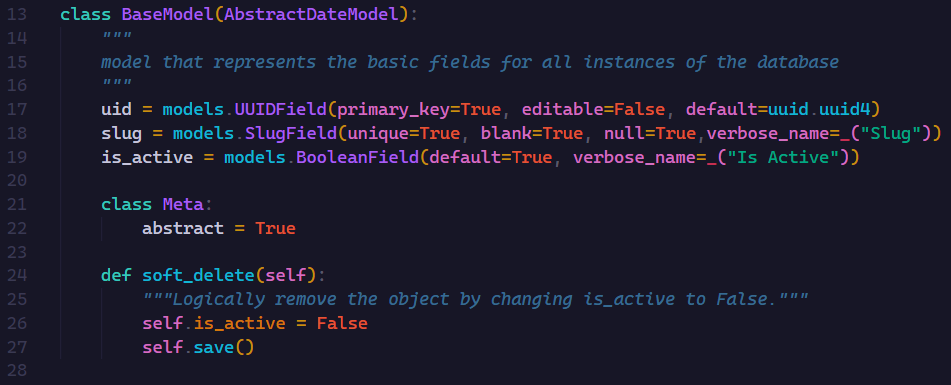
\includegraphics[width=0.8\textwidth]{images/codigo_template_method.png}
	\caption{Extracto de código que implementa el patrón \textit{Plantilla Abstracta} (Fuente: elaboración propia).}
	\label{fig:codigo_template_method}
\end{figure}

\textbf{Patrón Fachada} permite simplificar la interacción con subsistemas complejos, encapsulando la lógica de manejo de mensajes y respuestas en clases específicas. Este patrón permite abstraer operaciones complejas, como el formateo de mensajes o la gestión de respuestas de un modelo de lenguaje, en una interfaz sencilla que puede ser utilizada por otras partes del sistema. La Figura \ref{fig:codigo_facade} muestra un ejemplo de la implementación de este patrón.\\
La relevancia del patrón \textit{Facade/Service} radica en su capacidad para reducir la complejidad del \textit{backend}, permitiendo que los controladores de \textit{Django REST Framework} se centren en la lógica de negocio mientras las clases de servicio manejan las operaciones más técnicas. Esto mejora la modularidad y facilita la integración con el sistema multiagente, asegurando que las respuestas generadas por el Microservicio MAS se procesen y entreguen al \textit{frontend} de manera eficiente.

\begin{figure}[htbp]
	\centering
	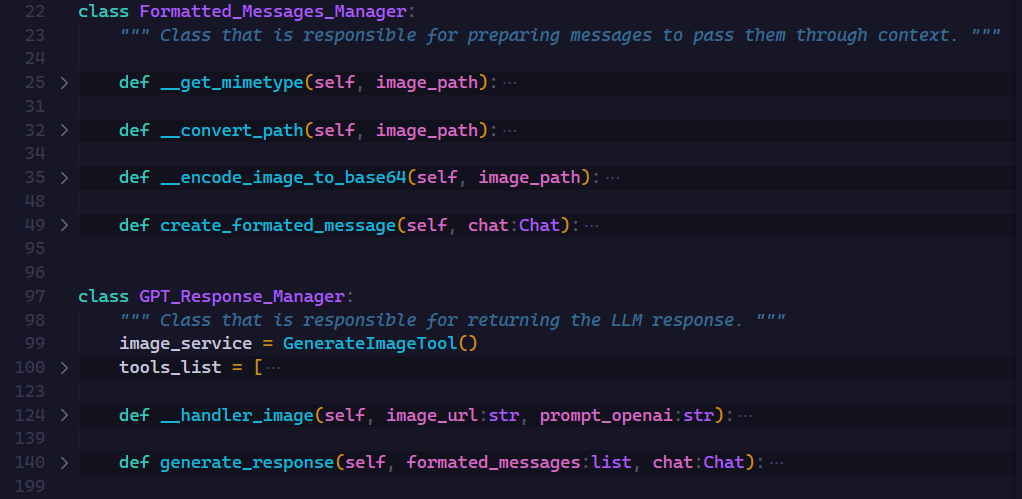
\includegraphics[width=0.8\textwidth]{images/fachada.PNG}
	\caption{Extracto de código que implementa el patrón \textit{Fachada} (Fuente: elaboración propia).}
	\label{fig:codigo_facade}
\end{figure}

El uso de estos patrones de diseño en el sistema multiagente y el \textit{backend} no solo asegura una implementación robusta y escalable, sino que también facilita la transformación de datos históricos del \textit{Diario de la Marina} en conocimiento estructurado, cumpliendo con los objetivos del proyecto.



\subsection{Interfaz Principal del Sistema}

La figura \ref{fig:interfaz} muestra la interfaz principal del sistema multiagente, diseñado para permitir la interacción en lenguaje natural con datos históricos del \textit{Diario de la Marina}. A continuación, se detalla cada uno de los componentes numerados de la interfaz:

\begin{figure}[h!]
	\centering
	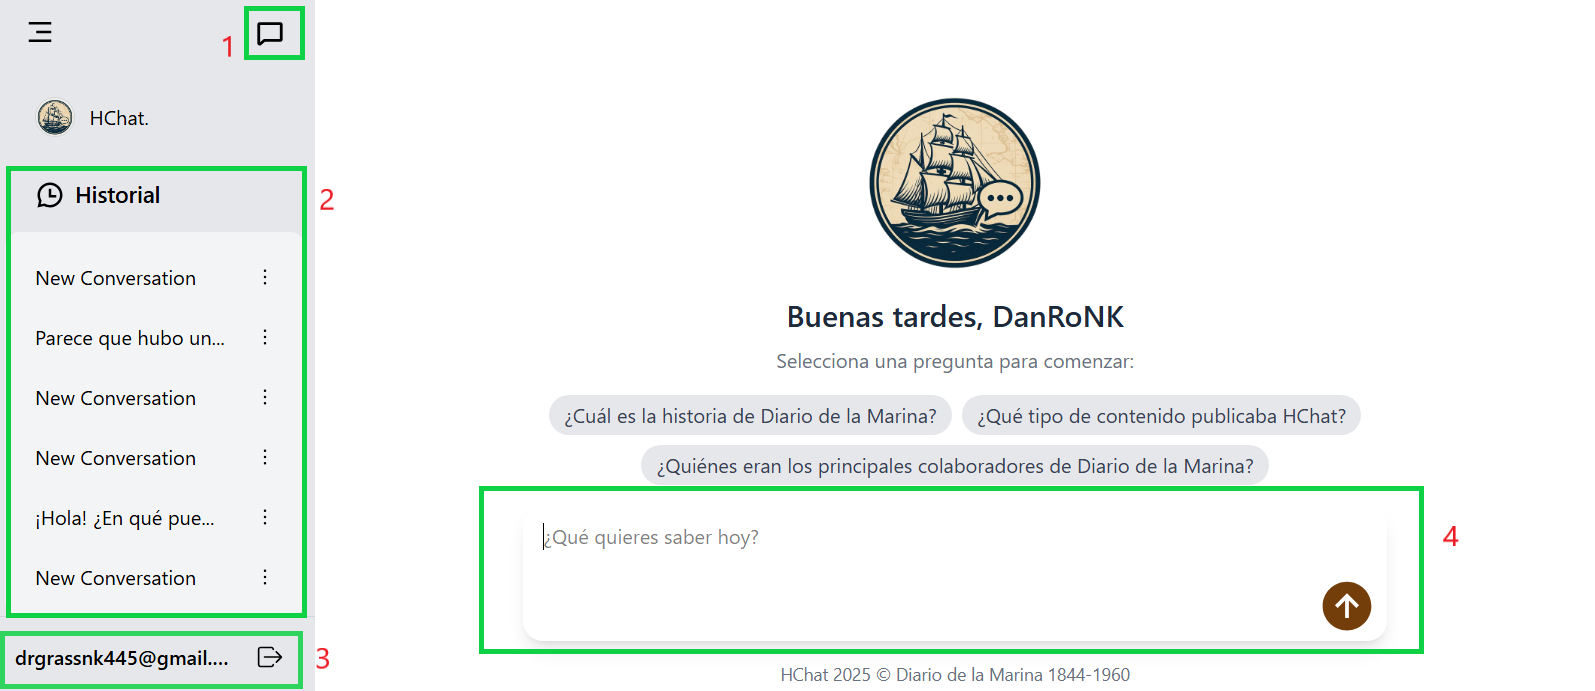
\includegraphics[width=1\textwidth]{images/interfaz1.png}
	\caption{Interfaz principal del chat con el sistema multiagente (Fuente: elaboración propia)}
	\label{fig:interfaz}
\end{figure}

\begin{enumerate}[label=\textbf{\arabic*.}]
	\item \textbf{Botón de Nuevo Chat}: ubicado en la parte superior izquierda, este botón permite al usuario iniciar una nueva conversación. Al activarse, se borra la conversación actual y se prepara el sistema para recibir una nueva consulta.
	
	\item \textbf{Panel de Historial de Conversaciones}: muestra una lista cronológica de conversaciones anteriores. Cada elemento incluye el título de la conversación (asignado automáticamente o manualmente) y un menú contextual para acciones como renombrar o eliminar. Esta sección permite retomar diálogos previos de forma eficiente.
	
	\item \textbf{Información del Usuario}: en la parte inferior del panel lateral se muestra el correo electrónico del usuario autenticado. Incluye un botón para copiar fácilmente la dirección, facilitando su reutilización o verificación de sesión.
	
	\item \textbf{Área de Entrada de Consulta}: permite al usuario redactar y enviar preguntas o mensajes. El campo de texto cuenta con una sugerencia que invita a interactuar: \textit{¿Qué quieres saber hoy?}. Incluye un botón de envío que ejecuta la solicitud hacia el sistema conversacional.
	
\end{enumerate}

\subsection{Diagrama de despliege}

Los diagramas de despliegue muestran cómo los componentes de software se despliegan
físicamente en los procesadores; es decir, el diagrama de despliegue muestra el hardware
y el software en el sistema, así como el middleware~\footnote{Middleware, también conocido como lógica de intercambio de información entre aplicaciones o agente intermedio, es un sistema de software que ofrece servicios y funciones comunes para las aplicaciones.} usado para conectar los diferentes
componentes en el sistema. En esencia, los diagramas de despliegue se pueden considerar
como una forma de definir y documentar el entorno objetivo~\cite{sommerville2011software}.\\
A continuación, la figura~\ref{fig:despliege}. muestra el diagrama correspondiente al sistema propuesto.\\
\textbf{Nodos:} elementos de procesamiento con al menos un procesador, memoria, y posiblemente otros dispositivos.\\
\textbf{Dispositivos:} nodos estereotipados sin capacidad de procesamiento en el nivel de abstracción que se modela.\\
\textbf{Conectores:} expresa el tipo de conector o protocolo utilizado entre el resto de los elementos del modelo.\\

\begin{figure}[h!]
	\centering
	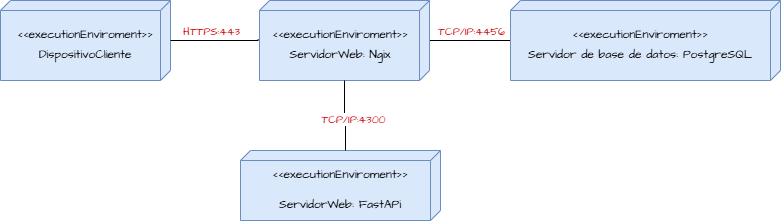
\includegraphics[width=1\textwidth]{images/despliege.drawio.png}
	\caption{Representación del modelo de despliegue. (Fuente: elaboración propia).}
	\label{fig:despliege}
\end{figure}

\textbf{Dispositivo del cliente}: Se refiere al conjunto de todos los clientes que consumirán el software desde sus computadoras. La máquina cliente necesita de pocas
prestaciones; teniendo un navegador web (Chrome, Mozilla Firefox, Internet Explorer,Opera), una RAM mínima de 4 GB, una tarjeta de red y un procesador mínimo de 3.3 GB podrá acceder al sistema y realizar las operaciones necesarias.\\
\textbf{Servidor Web}: Representa el servidor que se comunica con la PC Cliente mediante el protocolo HTTPS y además realiza peticiones al servidor de Bases de Datos mediante el protocolo TCP/IP, es el encargado de la presentación del repositorio, debe estar compuesto de 32 GB de RAM, 1 TB de almacenamiento, un procesador de 3.3 GHz o superior, una tarjeta de red, servidor web Nginx o Treafic con Docker.\\
\textbf{Servidor de BD}: Es el servidor, dedicado a almacenar y proveer datos necesarios para el funcionamiento de la aplicación web. es el encargado de almacenar la información generada del
sistema, para el correcto funcionamiento del repositorio es necesario que posea PostgreSQL, una RAM mínima de 4 GB, un procesador mínimo de 3.3 GHz y un disco duro de 1 TB.

\section*{Conclusiones del capítulo}
\addcontentsline{toc}{section}{Conclusiones}

El capítulo 2 presenta un enfoque metodológico y técnico para abordar la interpretación de datos históricos no estructurados del Diario de la Marina, integrando metodologías ágiles, arquitecturas multiagente y tecnologías emergentes. La aplicación de Extreme Programming permitió adaptar el desarrollo a las necesidades identificadas en usuarios especializados, como historiadores, priorizando la corrección de errores de OCR y la contextualización de respuestas. La arquitectura propuesta, basada en microservicios y agentes especializados (Moderador, Recuperador, Contextualizador), mostró potencial para gestionar la complejidad de los datos mediante la coordinación de tareas como la recuperación semántica con FAISS y la generación de visualizaciones dinámicas.

La selección de herramientas como LangChain, modelos de embeddings y bases de datos vectoriales contribuyó a optimizar la precisión en el procesamiento de consultas, mientras que patrones de diseño como Singleton y Cadena de Responsabilidad reforzaron la mantenibilidad del sistema. La interfaz, diseñada para facilitar la interacción con usuarios no técnicos, combinó un historial de conversaciones y visualizaciones gráficas, evidenciando la viabilidad de transformar datos históricos en conocimiento accesible.

Este enfoque sugiere un avance en el campo de la informática histórica, al proponer un marco replicable que integra sistemas multiagente con IA generativa, adaptable a otros contextos de patrimonio digital. Las decisiones técnicas, respaldadas por un proceso iterativo y centrado en el usuario, reflejan una solución equilibrada entre innovación y aplicabilidad práctica, sentando bases para futuras validaciones experimentales y ampliaciones del sistema.
 % Capítulo 2
	\chapter{Validación y Análisis de Resultados}
\label{chap:chapter3}

 % Capítulo 3
	\conclusions
\label{chap:conclusiones-generales}

%El presente trabajo de diploma concluye con resultados significativos en el desarrollo de un sistema multiagente conversacional, capaz de interpretar y contextualizar datos históricos no estructurados del transporte marítimo, extraídos del Diario de la Marina.
%\begin{itemize}
	%\item Se logró construir un marco conceptual sólido que integró tecnologías clave como OCR, LLM, sistemas multiagente, RAG, modelos de embeddings y bases de datos vectoriales. Este marco permitió abordar con eficacia la complejidad de los documentos históricos, facilitando su digitalización, estructuración y comprensión automatizada.
	%\item Los resultados del análisis comparativo con herramientas conversacionales existentes evidenciaron que las soluciones generalistas presentan limitaciones notables frente a textos históricos con errores de OCR. En contraste, el sistema propuesto demostró una mayor capacidad para ofrecer respuestas contextualizadas, ajustadas a las particularidades del dominio histórico estudiado.
	%\item La arquitectura implementada, basada en microservicios y patrones de diseño bien establecidos, permitió alcanzar una solución flexible, escalable y fácilmente mantenible. El sistema respondió de manera efectiva a los requisitos funcionales y no funcionales, superando los estándares iniciales en modularidad y organización del código.
	%\item El sistema fue capaz de transformar datos históricos crudos en información útil mediante respuestas textuales coherentes y visualizaciones gráficas precisas. Esta funcionalidad fue validada a través de múltiples escenarios de prueba, confirmando su utilidad como herramienta para la consulta y análisis de fuentes históricas complejas.
	%\item La estrategia de pruebas aplicada permitió identificar y resolver errores críticos antes de la fase de despliegue. Se alcanzó un índice de satisfacción del usuario (ISG) de 0.8, lo cual valida positivamente la experiencia de uso. Además, se evidenció un buen desempeño del componente de IA en la generación de respuestas, con oportunidades identificadas para optimizaciones futuras.
%\end{itemize}

A partir del desarrollo de la presente investigación, se constata el cumplimiento de los objetivos específicos planteados, los cuales guiaron de manera sistemática la construcción de un sistema multiagente conversacional orientado a la interpretación y contextualización de datos históricos no estructurados provenientes del \textit{Diario de la Marina}.

\begin{itemize}
	\item El análisis de los referentes teóricos y metodológicos permitió construir un andamiaje conceptual sólido que integró tecnologías fundamentales como el Reconocimiento Óptico de Caracteres (OCR), los modelos de lenguaje de gran escala (LLM), los sistemas multiagente, las arquitecturas RAG, los modelos de \textit{embeddings} y las bases de datos vectoriales. Este marco teórico facilitó la comprensión de las problemáticas asociadas al tratamiento de datos históricos no estructurados y sustentó las decisiones técnicas adoptadas en la propuesta de solución.
	
	\item Se desarrolló una arquitectura modular y escalable, que permitió definir claramente los componentes funcionales, sus responsabilidades, interacciones y flujos de trabajo. Este diseño se apoyó en el uso de patrones arquitectónicos y de diseño reconocidos, lo que favoreció la coherencia estructural del sistema y su mantenibilidad a largo plazo.
	
	\item Se implementó una solución tecnológica basada en una arquitectura de microservicios que articula un \textit{frontend} en React, un \textit{backend} en \textit{Django REST Framework} y un microservicio especializado construido con \textit{FastAPI}. Esta arquitectura posibilitó la coordinación efectiva entre agentes inteligentes encargados de la recuperación, contextualización y generación de respuestas a partir de datos históricos digitalizados. El sistema demostró capacidad para transformar datos no estructurados en conocimiento accesible y contextualizado, tanto en formato textual como visual.
	
	\item Finalmente, en cuanto a la validación del sistema desarrollado, se llevaron a cabo pruebas exhaustivas que incluyeron pruebas unitarias, funcionales, de rendimiento y de seguridad. Los resultados evidenciaron un cumplimiento satisfactorio de los requisitos definidos, así como una alta precisión en la interpretación de consultas en lenguaje natural. No obstante, se identificaron desafíos asociados a la latencia en la respuesta, inherentes a la naturaleza síncrona de los procesos de inferencia.
\end{itemize}

En síntesis, la presente investigación demuestra la viabilidad técnica y metodológica de emplear sistemas multiagente conversacionales, integrados con modelos de lenguaje y técnicas de recuperación aumentada por generación, para revitalizar y poner en valor archivos históricos digitalizados mediante interacciones en lenguaje natural.
 % Conclusiones
	\suggestions
\begin{itemize}
	\item Recomendaci�n 1
	
	\item Recomendaci�n 2 ...
	
	\item Recomendaci�n n
\end{itemize} % Recomendaciones
	
	
	% ============================
	% ANEXOS Y REFERENCIAS
	% ============================
	\appendix
	\appendixes

\renewcommand{\appendixname}{Anexo}
\renewcommand{\appendixtocname}{Anexos}
\renewcommand{\appendixpagename}{Anexos}
%\newcounter{anexo1}
%\setcounter{anexo1}{1}
\begin{addendum}
	
	\chapter{Historias de Usuario}
	% ==========================================
	% Gestión de Usuarios y Autenticación
	% ==========================================
	
	\begin{userstory}[hu:01]
		\storyname{Registrar una nueva cuenta de usuario}
		\storyuser{Visitante del sitio web}
		\storyiter{1} % Iteración estimada
		\storypriority{Alta} % Basado en RF1
		\storyrisk{Bajo}
		\storypoints{1 semana} % Estimación basada en ejemplo
		\storyprogrammer{Daniel Rojas Grass} % Manteniendo el nombre del ejemplo
		\storydescription{
			Como visitante del sitio web, debe poder registrar una nueva cuenta proporcionando su dirección de correo electrónico, nombre de usuario y una contraseña segura, para crear una cuenta personal que la permita acceder a las funcionalidades de consulta y visualización del archivo histórico y guardar su historial de conversaciones. (Corresponde principalmente a RF1)
			
			\textbf{Precondiciones:}
			\begin{itemize}
				\item El visitante no tiene una sesión activa.
				\item El visitante se encuentra en la página o sección de registro del sitio web.
				\item El \textit{backend} está operativo y accesible.
			\end{itemize}
			
			\textbf{Flujo de acción:}
			\begin{enumerate}
				\item Visitante ingresa dirección de correo electrónico, nombre de usuario, contraseña y confirmación de contraseña en el formulario de la sección registrar cuenta.
				\item Visitante envía el formulario.
				\item El sitio web valida formato básico (e.g., dirección de correo electrónico válido, contraseñas coinciden, nombre de usuario único).
				\item El sitio web envía los datos al endpoint de registro del \textit{backend}.
				\item El \textit{backend} valida los datos (e.g., dirección de correo electrónico no existente,nombre de usuario no existente, complejidad de contraseña) y crea el usuario en la base de datos de forma segura.
				\item El \textit{backend} retorna una respuesta de éxito o error al frontend.
				\item El \textit{frontend} muestra un mensaje apropiado al usuario (éxito o error específico).
			\end{enumerate}
		}
		\storyobservation{
			Implementar validación de fortaleza de contraseña en \textit{frontend} y \textit{backend}. Asegurar almacenamiento seguro de contraseñas (hashing). Los mensajes de error deben ser claros (e.g., 'El correo electrónico ya está registrado', "Las contraseñas no coinciden").
		}
		\storyinterface{ % Inicio del contenido de storyinterface
			Formulario de registro del sitio web: % Texto descriptivo inicial
			\par\medskip % Añade un pequeño espacio vertical
			\begin{center} % Para centrar la imagen
				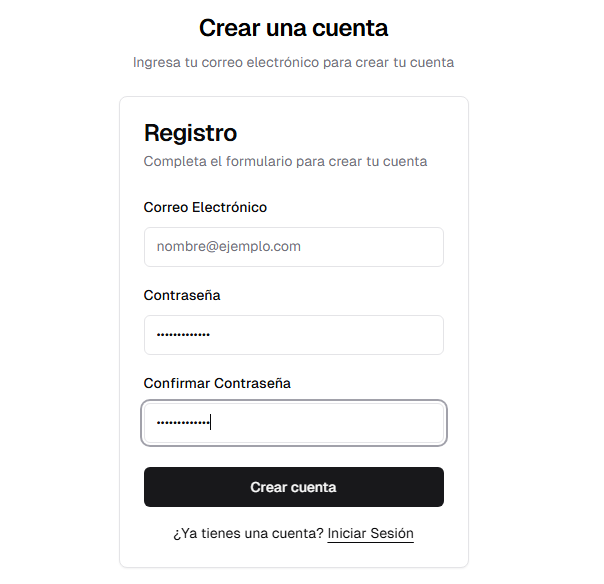
\includegraphics[width=0.6\textwidth]{images/create.PNG} % Imagen del ejemplo
			\end{center}
			\medskip % Espacio después de la imagen
		}
		
		
	\end{userstory}
	
	\begin{userstory}[hu:02]
		\storyname{Iniciar sesión en el sistema}
		\storyuser{Usuario registrado}
		\storyiter{1} % Iteración estimada
		\storypriority{Alta} % Basado en RF2
		\storyrisk{Bajo}
		\storypoints{1 semana} % Estimación basada en ejemplo
		\storyprogrammer{Daniel Rojas Grass}
		\storydescription{
			Como usuario registrado, debe poder iniciar sesión utilizando su correo electrónico y contraseña previamente registrados, mi historial de conversaciones y utilizar las capacidades completas del sistema de chat. (Corresponde principalmente a RF2, RF4)
			
			\textbf{Precondiciones:}
			\begin{itemize}
				\item El usuario tiene una cuenta previamente registrada en el sistema.
				\item El usuario no tiene una sesión activa.
				\item El usuario se encuentra en la página o sección de inicio de sesión del sitio web.
				\item El \textit{backend} está operativo y accesible.
			\end{itemize}
			
			\textbf{Flujo de acción:}
			\begin{enumerate}
				\item Usuario ingresa su dirección de correo electrónico y contraseña en el formulario del sitio web.
				\item Usuario envía el formulario.
				\item El sitio web envía las credenciales al \textit{endpoint} de autenticación del \textit{backend}.
				\item El \textit{backend} verifica las credenciales contra la base de datos.
				\item Si las credenciales son válidas, el \textit{backend} genera un token de sesión (e.g., JWT) y lo retorna al \textit{frontend}.
				\item Si las credenciales son inválidas, el backend retorna un error de autenticación.
				\item El \textit{frontend} almacena el token de sesión de forma segura (e.g., localStorage, sessionStorage o cookie HttpOnly).
				\item Si el inicio de sesión es exitoso, el \textit{frontend} redirige al usuario a la interfaz principal del chat. Si falla, muestra un mensaje de error ("Credenciales incorrectas").
			\end{enumerate}
		}
		\storyobservation{
			Utilizar HTTPS para la comunicación. Implementar medidas contra ataques de fuerza bruta (e.g., límites de intentos). El manejo del token en el \textit{frontend} debe seguir las mejores prácticas de seguridad.
		}
		\storyinterface{
			Formulario de inicio de sesión del sitio web:
			\par\medskip % Añade un pequeño espacio vertical
			\begin{center} % Para centrar la imagen
				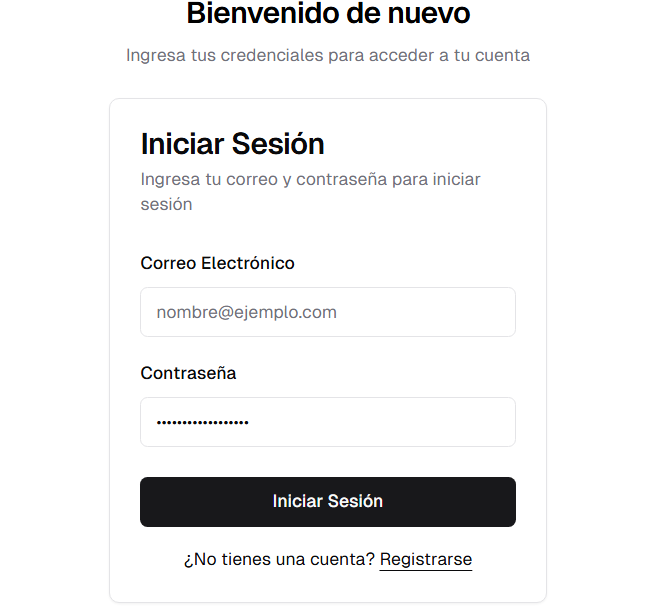
\includegraphics[width=0.6\textwidth]{images/loguin.PNG} % Imagen del ejemplo
			\end{center}
			\medskip
		}
		
	\end{userstory}
	
	\begin{userstory}[hu:03]
		\storyname{Cerrar sesión del sistema}
		\storyuser{Usuario autenticado}
		\storyiter{1} % Iteración estimada
		\storypriority{Media} % Basado en RF3
		\storyrisk{Bajo}
		\storypoints{0.5 semanas} % Estimación basada en ejemplo
		\storyprogrammer{Daniel Rojas Grass}
		\storydescription{
			Como usuario autenticado, debe disponer de una opción clara para cerrar su sesión activa, para asegurar la privacidad de su cuenta y finalizar su interacción con el sistema de forma segura. (Corresponde principalmente a RF3)
			
			\textbf{Precondiciones:}
			\begin{itemize}
				\item El usuario tiene una sesión activa (posee un token válido).
				\item El usuario está en la interfaz principal del sistema.
			\end{itemize}
			
			\textbf{Flujo de acción:}
			\begin{enumerate}
				\item Usuario hace clic en el botón o enlace 'Cerrar Sesión'.
				\item El \textit{frontend} elimina el token de sesión almacenado localmente.
				\item (Recomendado) El \textit{frontend} envía una solicitud al \textit{backend} para invalidar el token en el servidor (si se usa una blacklist de tokens).
				\item El \textit{frontend} redirige al usuario a la página de inicio de sesión o a una página pública principal.
				\item Cualquier intento posterior de acceder a rutas protegidas con el token antiguo debe fallar.
			\end{enumerate}
		}
		\storyobservation{
			El botón de cerrar sesión debe ser fácilmente accesible en la interfaz de usuario autenticado.
		}
		\storyinterface{Botón cerrar sesión en el sitio web:
			\par\medskip % Añade un pequeño espacio vertical
			\begin{center} % Para centrar la imagen
				
\includegraphics[width=0.6\textwidth]{images/cerrar.PNG} % Imagen del ejemplo
			\end{center}
		}
		
	\end{userstory}
	
	% ==========================================
	% Gestión de Conversaciones
	% ==========================================
	
	\begin{userstory}[hu:04]
		\storyname{Iniciar una nueva conversación}
		\storyuser{Usuario autenticado}
		\storyiter{2} % Iteración estimada
		\storypriority{Alta} % Basado en RF5
		\storyrisk{Bajo}
		\storypoints{0.5 semanas} % Estimación basada en ejemplo
		\storyprogrammer{Daniel Rojas Grass}
		\storydescription{
			Como usuario autenticado, debe poder iniciar una nueva conversación de chat en cualquier momento, para realizar consultas sobre temas distintos sin mezclar las interacciones o para empezar una nueva conversación si lo necesita. (Corresponde principalmente a RF5)
			
			\textbf{Precondiciones:}
			\begin{itemize}
				\item El usuario tiene una sesión activa.
				\item El usuario se encuentra en la interfaz principal del chat.
			\end{itemize}
			
			\textbf{Flujo de acción:}
			\begin{enumerate}
				\item Usuario hace clic en la opción "Nueva Conversación" (o icono '+').
				\item El \textit{frontend} limpia el área de visualización del chat actual.
				\item El \textit{frontend} establece un estado interno que indica que la próxima consulta pertenece a una nueva conversación (puede no requerir llamada inmediata al \textit{backend}).
				\item Opcionalmente, el \textit{frontend} puede asignar un ID temporal a la nueva conversación hasta que se envíe el primer mensaje.
				\item La interfaz se muestra lista para recibir la primera consulta de la nueva conversación.
			\end{enumerate}
		}
		\storyobservation{
			La acción debe ser visualmente clara y distinguible de seleccionar una conversación existente. El estado de "nueva conversación" debe manejarse correctamente hasta el primer envío.
		}
		\storyinterface{Botón nueva conversación en el sitio web:
			\par\medskip % Añade un pequeño espacio vertical
			\begin{center} % Para centrar la imagen
				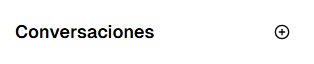
\includegraphics[width=0.6\textwidth]{images/newConversation.PNG} % Imagen del ejemplo
			\end{center}
			\medskip
		}
		
	\end{userstory}
	
	\begin{userstory}[hu:05]
		\storyname{Ver historial de conversaciones}
		\storyuser{Usuario autenticado}
		\storyiter{2} % Iteración estimada
		\storypriority{Media} % Basado en RF6
		\storyrisk{Bajo}
		\storypoints{1 semana} % Estimación basada en ejemplo
		\storyprogrammer{Daniel Rojas Grass}
		\storydescription{
			Como usuario autenticado, debe ver una lista organizada de sus conversaciones anteriores (por ejemplo, con un título autogenerado o fecha), para poder identificar y acceder fácilmente a interacciones pasadas. (Corresponde principalmente a RF6)
			
			\textbf{Precondiciones:}
			\begin{itemize}
				\item El usuario tiene una sesión activa.
				\item El \textit{backend} y la base de datos que almacena el historial están operativos.
			\end{itemize}
			
			\textbf{Flujo de acción:}
			\begin{enumerate}
				\item El \textit{frontend} (al cargar la interfaz principal o al interactuar con un panel de historial) solicita la lista de conversaciones del usuario al \textit{backend}.
				\item El backend consulta la base de datos para obtener los metadatos de las conversaciones asociadas al usuario autenticado (ID, título/fecha, última actualización).
				\item El \textit{backend} retorna la lista de conversaciones al \textit{frontend}.
				\item El \textit{frontend} muestra la lista en un panel lateral o sección designada, permitiendo al usuario ver los identificadores de cada conversación.
			\end{enumerate}
		}
		\storyobservation{
			Considerar paginación si el historial puede ser muy largo. La generación de títulos/identificadores debe ser útil (e.g., basado en la primera consulta). La lista debe actualizarse si se crea o elimina una conversación.
		}
		\storyinterface{Panel/Sección de Historial en el sitio web:
			\par\medskip % Añade un pequeño espacio vertical
			\begin{center} % Para centrar la imagen
				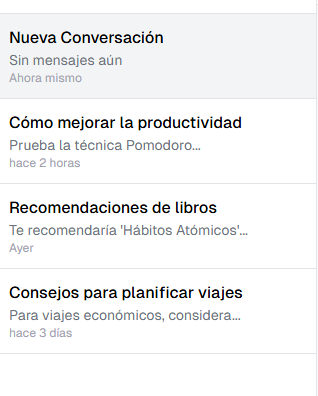
\includegraphics[width=0.4\textwidth]{images/histo.PNG} % Imagen del ejemplo
			\end{center}
			\medskip
		}
		
	\end{userstory}
	
	\begin{userstory}[hu:06]
		\storyname{Abrir una conversación del historial}
		\storyuser{Usuario autenticado}
		\storyiter{2} % Iteración estimada
		\storypriority{Media} % Basado en RF7
		\storyrisk{Bajo}
		\storypoints{1 semana} % Estimación basada en ejemplo
		\storyprogrammer{Daniel Rojas Grass}
		\storydescription{
			Como usuario autenticado, debe poder seleccionar una conversación específica de su historial listado, para cargar su contenido completo (consultas y respuestas) en la interfaz principal del chat y, opcionalmente, continuarla. (Corresponde principalmente a RF7)
			
			\textbf{Precondiciones:}
			\begin{itemize}
				\item El usuario tiene una sesión activa.
				\item El usuario está viendo la lista de su historial de conversaciones (HU:05).
				\item El \textit{backend} y la base de datos que almacena el historial están operativos.
			\end{itemize}
			
			\textbf{Flujo de acción:}
			\begin{enumerate}
				\item Usuario hace clic en una conversación específica en la lista del historial.
				\item El \textit{frontend} envía una solicitud al \textit{backend} pidiendo el contenido completo de la conversación seleccionada (pasando su ID).
				\item El \textit{backend} recupera todas las consultas y respuestas asociadas a esa conversación para ese usuario.
				\item El \textit{backend} retorna el historial completo de mensajes de esa conversación al \textit{frontend}.
				\item El \textit{backend} limpia el área de chat actual y muestra los mensajes recuperados en el orden correcto.
				\item El \textit{backend} establece la conversación seleccionada como la "conversación activa" actual.
				\item La interfaz permite al usuario añadir nuevas consultas a esta conversación activa.
			\end{enumerate}
		}
		\storyobservation{
			La carga debe ser eficiente, especialmente para conversaciones largas. La interfaz debe indicar claramente cuál conversación del historial está activa.
		}
		\storyinterface{Interacción con lista de historial y chat principal en el sitio web:
			\par\medskip % Añade un pequeño espacio vertical
			\begin{center} % Para centrar la imagen
				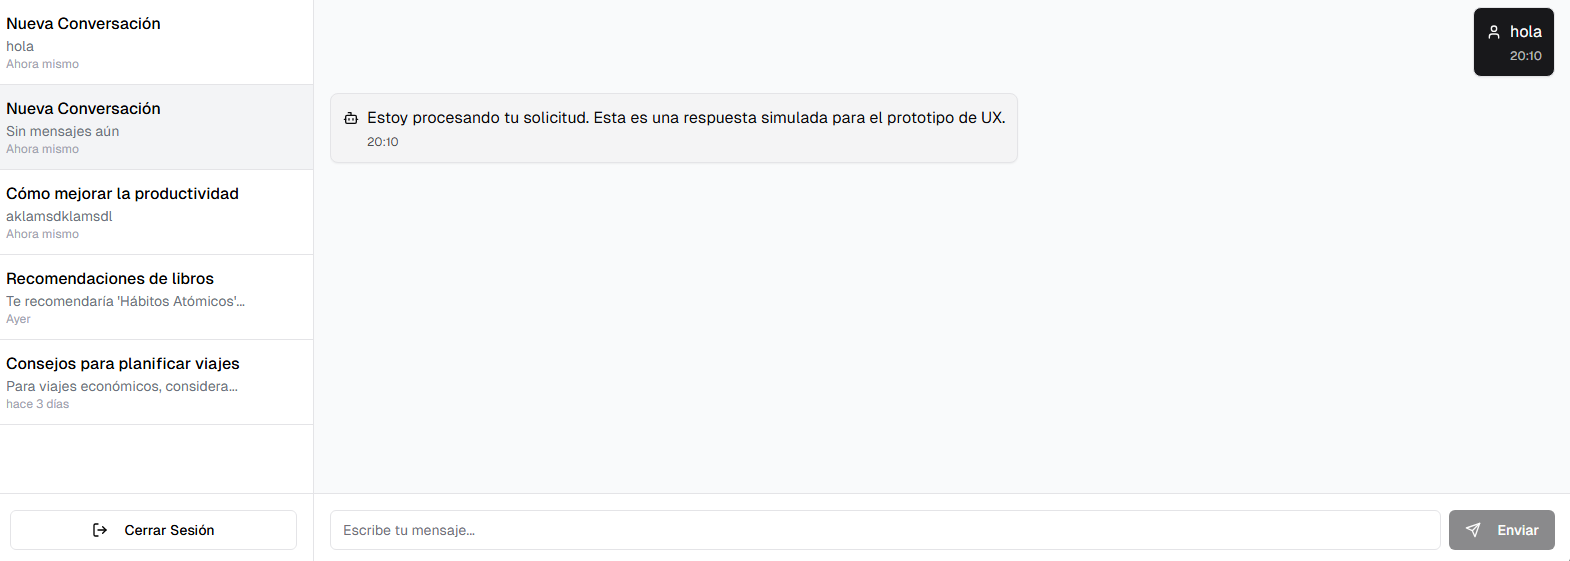
\includegraphics[width=0.6\textwidth]{images/lista.PNG} % Imagen del ejemplo
			\end{center}
			\medskip
		}
		
	\end{userstory}
	
	\begin{userstory}[hu:07]
		\storyname{Eliminar una conversación del historial}
		\storyuser{Usuario autenticado}
		\storyiter{3} % Iteración estimada
		\storypriority{Baja} % Basado en RF8
		\storyrisk{Bajo} % Riesgo de pérdida de datos si no hay confirmación
		\storypoints{1 semana} % Estimación basada en ejemplo
		\storyprogrammer{Daniel Rojas Grass}
		\storydescription{
			Como usuario autenticado, debe tener la opción de eliminar permanentemente una conversación específica de su historial, para mantener su historial limpio y relevante. (Corresponde principalmente a RF8)
			
			\textbf{Precondiciones:}
			\begin{itemize}
				\item El usuario tiene una sesión activa.
				\item El usuario está viendo la lista de su historial o tiene una conversación cargada que desea eliminar.
				\item El \textit{backend} y la base de datos que almacena el historial están operativos.
			\end{itemize}
			
			\textbf{Flujo de acción:}
			\begin{enumerate}
				\item Usuario hace clic en la opción "Eliminar" asociada a una conversación en la lista del historial (o en la conversación activa).
				\item El \textit{frontend} muestra un diálogo de confirmación ("¿Estás seguro de que quieres eliminar esta conversación? Esta acción no se puede deshacer.").
				\item Si el usuario confirma la eliminación:
				\begin{enumerate}
					\item El frontend envía una solicitud al backend DRF para eliminar la conversación (pasando su ID).
					\item El backend verifica que la conversación pertenece al usuario y la elimina de la base de datos.
					\item El backend retorna una respuesta de éxito al frontend.
					\item El frontend elimina la conversación de la lista visible en el historial.
					\item Si la conversación eliminada era la activa, el frontend limpia el área de chat o carga una conversación por defecto/nueva.
				\end{enumerate}
				\item Si el usuario cancela, no se realiza ninguna acción.
			\end{enumerate}
		}
		\storyobservation{
			La confirmación es crucial para prevenir eliminaciones accidentales. La eliminación debe ser lógicamente completa en el backend (borrado permanente).
		}
		\storyinterface{Opción de Eliminar en la lista de Historial o Chat activo:
			\par\medskip % Añade un pequeño espacio vertical
			\begin{center} % Para centrar la imagen
				
\includegraphics[width=0.6\textwidth]{images/eliminarC.PNG} % Imagen del ejemplo (asumiendo que muestra un icono/botón de eliminar)
			\end{center}
			\medskip
		}
		
	\end{userstory}
	
	
	\chapter{Targetas CRC}
		
		\begin{longtable}{|l|l|}
			\caption{Tarjeta CRC: Usuario} \label{tablacrc6} \\
			\hline
			\multicolumn{2}{|c|}{\textbf{Tarjeta CRC}} \\
			\hline
			\textbf{Clase} & \textbf{Usuario} \\
			\hline
			\parbox[t]{0.45\linewidth}{\textbf{Responsabilidades:} \\ 
				Proporcionar datos para registro (email, username, contraseña) \\ 
				Almacenar credenciales de forma segura \\ 
				Mantener información de sesión activa \\ 
				Asociar conversaciones al usuario} 
			& 
			\parbox[t]{0.45\linewidth}{\textbf{Colaboración:} \\ 
				Autenticador \\ 
				BaseDeDatos \\ 
				Conversación} \\
			\hline
		\end{longtable}
		
		\begin{longtable}{|l|l|}
			\caption{Tarjeta CRC: Autenticador} \label{tablacrc7} \\
			\hline
			\multicolumn{2}{|c|}{\textbf{Tarjeta CRC}} \\
			\hline
			\textbf{Clase} & \textbf{Autenticador} \\
			\hline
			\parbox[t]{0.45\linewidth}{\textbf{Responsabilidades:} \\ 
				Validar datos de registro (email único, contraseña fuerte) \\ 
				Autenticar credenciales de inicio de sesión \\ 
				Generar y gestionar tokens de sesión \\ 
				Finalizar sesiones activas} 
			& 
			\parbox[t]{0.45\linewidth}{\textbf{Colaboración:} \\ 
				Usuario \\ 
				BaseDeDatos \\ 
				Backend} \\
			\hline
		\end{longtable}
		
		\begin{longtable}{|l|l|}
			\caption{Tarjeta CRC: Conversación} \label{tablacrc8} \\
			\hline
			\multicolumn{2}{|c|}{\textbf{Tarjeta CRC}} \\
			\hline
			\textbf{Clase} & \textbf{Conversación} \\
			\hline
			\parbox[t]{0.45\linewidth}{\textbf{Responsabilidades:} \\ 
				Iniciar una nueva sesión de chat \\ 
				Almacenar consultas y respuestas \\ 
				Permitir continuación de una conversación existente \\ 
				Eliminar una conversación del historial} 
			& 
			\parbox[t]{0.45\linewidth}{\textbf{Colaboración:} \\ 
				Usuario \\ 
				Historial \\ 
				Backend \\ 
				BaseDeDatos} \\
			\hline
		\end{longtable}
		
		\begin{longtable}{|l|l|}
			\caption{Tarjeta CRC: Historial} \label{tablacrc9} \\
			\hline
			\multicolumn{2}{|c|}{\textbf{Tarjeta CRC}} \\
			\hline
			\textbf{Clase} & \textbf{Historial} \\
			\hline
			\parbox[t]{0.45\linewidth}{\textbf{Responsabilidades:} \\ 
				Listar todas las conversaciones de un usuario \\ 
				Proporcionar metadatos de conversaciones (título, fecha) \\ 
				Permitir selección de una conversación específica} 
			& 
			\parbox[t]{0.45\linewidth}{\textbf{Colaboración:} \\ 
				Usuario \\ 
				Conversación \\ 
				Backend \\ 
				BaseDeDatos} \\
			\hline
		\end{longtable}
		
		\begin{longtable}{|l|l|}
			\caption{Tarjeta CRC: Chat} \label{tablacrc10} \\
			\hline
			\multicolumn{2}{|c|}{\textbf{Tarjeta CRC}} \\
			\hline
			\textbf{Clase} & \textbf{Chat} \\
			\hline
			\parbox[t]{0.45\linewidth}{\textbf{Responsabilidades:} \\ 
				Mostrar la interfaz de chat activo \\ 
				Permitir ingreso de consultas en lenguaje natural \\ 
				Visualizar consultas y respuestas (texto e imágenes) \\ 
				Indicar estado de procesamiento} 
			& 
			\parbox[t]{0.45\linewidth}{\textbf{Colaboración:} \\ 
				Conversación \\ 
				Backend \\ 
				MicroservicioMAS} \\
			\hline
		\end{longtable}
		
		\begin{longtable}{|l|l|}
			\caption{Tarjeta CRC: Backend} \label{tablacrc11} \\
			\hline
			\multicolumn{2}{|c|}{\textbf{Tarjeta CRC}} \\
			\hline
			\textbf{Clase} & \textbf{Backend} \\
			\hline
			\parbox[t]{0.45\linewidth}{\textbf{Responsabilidades:} \\ 
				Gestionar endpoints REST para autenticación y chat \\ 
				Coordinar comunicación entre frontend y MicroservicioMAS \\ 
				Almacenar y recuperar datos de conversaciones \\ 
				Proteger rutas con autenticación} 
			& 
			\parbox[t]{0.45\linewidth}{\textbf{Colaboración:} \\ 
				Usuario \\ 
				Autenticador \\ 
				Conversación \\ 
				Historial \\ 
				Chat \\ 
				MicroservicioMAS \\ 
				BaseDeDatos} \\
			\hline
		\end{longtable}
		
		\begin{longtable}{|l|l|}
			\caption{Tarjeta CRC: BaseDeDatos} \label{tablacrc12} \\
			\hline
			\multicolumn{2}{|c|}{\textbf{Tarjeta CRC}} \\
			\hline
			\textbf{Clase} & \textbf{BaseDeDatos} \\
			\hline
			\parbox[t]{0.45\linewidth}{\textbf{Responsabilidades:} \\ 
				Almacenar datos de usuarios (credenciales, sesiones) \\ 
				Persistir conversaciones y su historial \\ 
				Proveer acceso a datos del \textit{Diario de la Marina} (vectorial y CSV)} 
			& 
			\parbox[t]{0.45\linewidth}{\textbf{Colaboración:} \\ 
				Usuario \\ 
				Autenticador \\ 
				Conversación \\ 
				Historial \\ 
				Backend \\ 
				Agente Recuperador (FAISS) \\ 
				Agente PandasAi} \\
			\hline
		\end{longtable}
		
		\begin{longtable}{|l|l|}
			\caption{Tarjeta CRC: MicroservicioMAS} \label{tablacrc13} \\
			\hline
			\multicolumn{2}{|c|}{\textbf{Tarjeta CRC}} \\
			\hline
			\textbf{Clase} & \textbf{MicroservicioMAS} \\
			\hline
			\parbox[t]{0.45\linewidth}{\textbf{Responsabilidades:} \\ 
				Recibir consultas del backend \\ 
				Coordinar agentes internos para procesar consultas \\ 
				Devolver respuestas procesadas (texto e imágenes) al backend} 
			& 
			\parbox[t]{0.45\linewidth}{\textbf{Colaboración:} \\ 
				Backend \\ 
				Agente Moderador \\ 
				Agente Recuperador (FAISS) \\ 
				Agente Contextualizador \\ 
				Agente de Validación \\ 
				Agente PandasAi} \\
			\hline
		\end{longtable}
		
		
		
		
\end{addendum}
 % Anexos
	
	% Bibliografía
	\bibliographystyle{IEEEtran}
	\bibliography{library} 
	%\printbibliography
	
\end{document}